% Created by tikzDevice version 0.11 on 2018-05-04 09:34:02
% !TEX encoding = UTF-8 Unicode
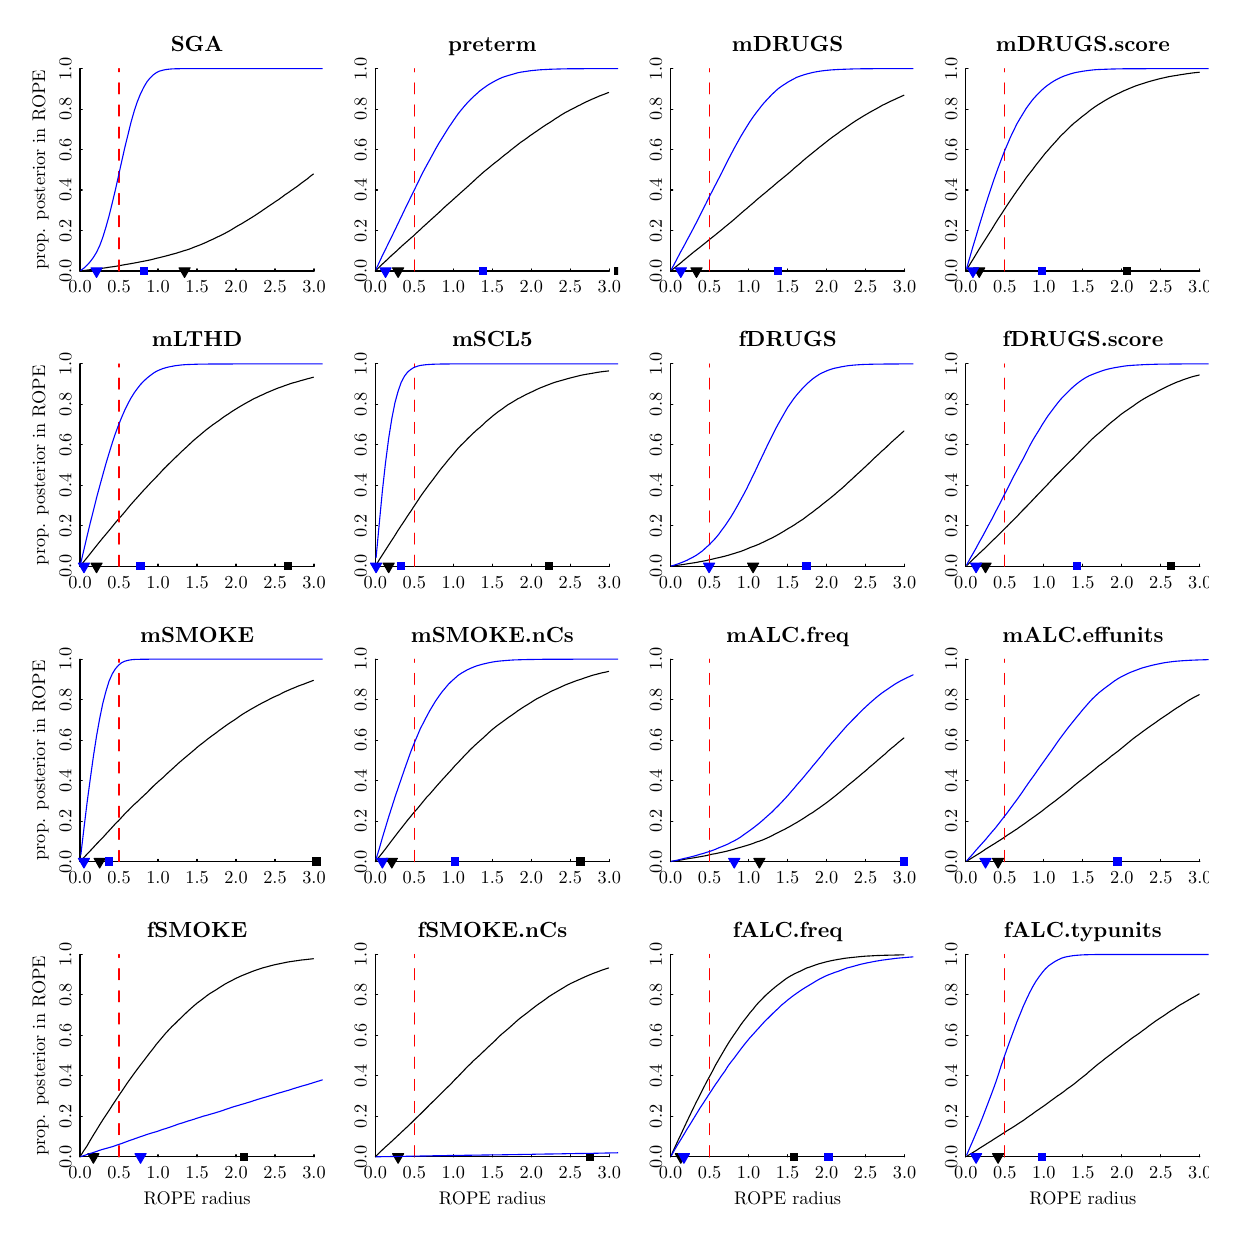
\begin{tikzpicture}[x=1pt,y=1pt]
\definecolor{fillColor}{RGB}{255,255,255}
\path[use as bounding box,fill=fillColor,fill opacity=0.00] (0,0) rectangle (426.79,426.79);
\begin{scope}
\path[clip] ( 15.84,335.93) rectangle (106.62,414.91);
\definecolor{drawColor}{RGB}{0,0,0}

\path[draw=drawColor,line width= 0.4pt,line join=round,line cap=round] ( 19.20,338.89) --
	( 20.34,339.03) --
	( 21.47,339.19) --
	( 22.61,339.33) --
	( 23.75,339.44) --
	( 24.88,339.58) --
	( 26.02,339.71) --
	( 27.15,339.87) --
	( 28.29,340.03) --
	( 29.42,340.22) --
	( 30.56,340.37) --
	( 31.70,340.53) --
	( 32.83,340.73) --
	( 33.97,340.94) --
	( 35.10,341.15) --
	( 36.24,341.34) --
	( 37.38,341.54) --
	( 38.51,341.74) --
	( 39.65,341.95) --
	( 40.78,342.18) --
	( 41.92,342.39) --
	( 43.06,342.62) --
	( 44.19,342.85) --
	( 45.33,343.13) --
	( 46.46,343.44) --
	( 47.60,343.69) --
	( 48.73,343.97) --
	( 49.87,344.27) --
	( 51.01,344.56) --
	( 52.14,344.89) --
	( 53.28,345.17) --
	( 54.41,345.53) --
	( 55.55,345.87) --
	( 56.69,346.25) --
	( 57.82,346.56) --
	( 58.96,346.98) --
	( 60.09,347.45) --
	( 61.23,347.88) --
	( 62.37,348.31) --
	( 63.50,348.79) --
	( 64.64,349.29) --
	( 65.77,349.83) --
	( 66.91,350.33) --
	( 68.04,350.91) --
	( 69.18,351.43) --
	( 70.32,352.00) --
	( 71.45,352.57) --
	( 72.59,353.18) --
	( 73.72,353.83) --
	( 74.86,354.55) --
	( 76.00,355.24) --
	( 77.13,355.84) --
	( 78.27,356.54) --
	( 79.40,357.23) --
	( 80.54,357.92) --
	( 81.67,358.63) --
	( 82.81,359.36) --
	( 83.95,360.13) --
	( 85.08,360.91) --
	( 86.22,361.68) --
	( 87.35,362.47) --
	( 88.49,363.23) --
	( 89.63,364.00) --
	( 90.76,364.74) --
	( 91.90,365.57) --
	( 93.03,366.43) --
	( 94.17,367.17) --
	( 95.31,368.00) --
	( 96.44,368.78) --
	( 97.58,369.57) --
	( 98.71,370.47) --
	( 99.85,371.30) --
	(100.98,372.11) --
	(102.12,373.07) --
	(103.26,373.93);
\end{scope}
\begin{scope}
\path[clip] (  0.00,320.09) rectangle (106.70,426.79);
\definecolor{drawColor}{RGB}{0,0,0}

\node[text=drawColor,anchor=base,inner sep=0pt, outer sep=0pt, scale=  0.79] at ( 61.23,418.12) {\bfseries SGA};

\node[text=drawColor,rotate= 90.00,anchor=base,inner sep=0pt, outer sep=0pt, scale=  0.66] at (  6.34,375.42) {prop. posterior in ROPE};
\end{scope}
\begin{scope}
\path[clip] (  0.00,  0.00) rectangle (426.79,426.79);
\definecolor{drawColor}{RGB}{0,0,0}

\path[draw=drawColor,line width= 0.4pt,line join=round,line cap=round] ( 18.92,338.86) -- (103.47,338.86);

\path[draw=drawColor,line width= 0.4pt,line join=round,line cap=round] ( 18.92,338.86) -- ( 18.92,339.65);

\path[draw=drawColor,line width= 0.4pt,line join=round,line cap=round] ( 33.01,338.86) -- ( 33.01,339.65);

\path[draw=drawColor,line width= 0.4pt,line join=round,line cap=round] ( 47.10,338.86) -- ( 47.10,339.65);

\path[draw=drawColor,line width= 0.4pt,line join=round,line cap=round] ( 61.20,338.86) -- ( 61.20,339.65);

\path[draw=drawColor,line width= 0.4pt,line join=round,line cap=round] ( 75.29,338.86) -- ( 75.29,339.65);

\path[draw=drawColor,line width= 0.4pt,line join=round,line cap=round] ( 89.38,338.86) -- ( 89.38,339.65);

\path[draw=drawColor,line width= 0.4pt,line join=round,line cap=round] (103.47,338.86) -- (103.47,339.65);

\node[text=drawColor,anchor=base,inner sep=0pt, outer sep=0pt, scale=  0.66] at ( 18.92,330.94) {0.0};

\node[text=drawColor,anchor=base,inner sep=0pt, outer sep=0pt, scale=  0.66] at ( 33.01,330.94) {0.5};

\node[text=drawColor,anchor=base,inner sep=0pt, outer sep=0pt, scale=  0.66] at ( 47.10,330.94) {1.0};

\node[text=drawColor,anchor=base,inner sep=0pt, outer sep=0pt, scale=  0.66] at ( 61.20,330.94) {1.5};

\node[text=drawColor,anchor=base,inner sep=0pt, outer sep=0pt, scale=  0.66] at ( 75.29,330.94) {2.0};

\node[text=drawColor,anchor=base,inner sep=0pt, outer sep=0pt, scale=  0.66] at ( 89.38,330.94) {2.5};

\node[text=drawColor,anchor=base,inner sep=0pt, outer sep=0pt, scale=  0.66] at (103.47,330.94) {3.0};

\path[draw=drawColor,line width= 0.4pt,line join=round,line cap=round] ( 18.92,338.86) -- ( 18.92,411.99);

\path[draw=drawColor,line width= 0.4pt,line join=round,line cap=round] ( 18.92,338.86) -- ( 19.71,338.86);

\path[draw=drawColor,line width= 0.4pt,line join=round,line cap=round] ( 18.92,353.48) -- ( 19.71,353.48);

\path[draw=drawColor,line width= 0.4pt,line join=round,line cap=round] ( 18.92,368.11) -- ( 19.71,368.11);

\path[draw=drawColor,line width= 0.4pt,line join=round,line cap=round] ( 18.92,382.74) -- ( 19.71,382.74);

\path[draw=drawColor,line width= 0.4pt,line join=round,line cap=round] ( 18.92,397.36) -- ( 19.71,397.36);

\path[draw=drawColor,line width= 0.4pt,line join=round,line cap=round] ( 18.92,411.99) -- ( 19.71,411.99);

\node[text=drawColor,rotate= 90.00,anchor=base,inner sep=0pt, outer sep=0pt, scale=  0.66] at ( 15.75,338.86) {0.0};

\node[text=drawColor,rotate= 90.00,anchor=base,inner sep=0pt, outer sep=0pt, scale=  0.66] at ( 15.75,353.48) {0.2};

\node[text=drawColor,rotate= 90.00,anchor=base,inner sep=0pt, outer sep=0pt, scale=  0.66] at ( 15.75,368.11) {0.4};

\node[text=drawColor,rotate= 90.00,anchor=base,inner sep=0pt, outer sep=0pt, scale=  0.66] at ( 15.75,382.74) {0.6};

\node[text=drawColor,rotate= 90.00,anchor=base,inner sep=0pt, outer sep=0pt, scale=  0.66] at ( 15.75,397.36) {0.8};

\node[text=drawColor,rotate= 90.00,anchor=base,inner sep=0pt, outer sep=0pt, scale=  0.66] at ( 15.75,411.99) {1.0};
\end{scope}
\begin{scope}
\path[clip] ( 15.84,335.93) rectangle (106.62,414.91);
\definecolor{drawColor}{RGB}{0,0,0}

\path[draw=drawColor,line width= 0.4pt,line join=round,line cap=round] (131.65,338.86) --
	(131.65,411.99);
\definecolor{drawColor}{RGB}{255,0,0}

\path[draw=drawColor,line width= 0.4pt,dash pattern=on 4pt off 4pt ,line join=round,line cap=round] ( 33.01,338.86) --
	( 33.01,411.99);
\definecolor{fillColor}{RGB}{0,0,0}

\path[fill=fillColor] (130.17,337.37) --
	(133.14,337.37) --
	(133.14,340.34) --
	(130.17,340.34) --
	cycle;
\definecolor{drawColor}{RGB}{0,0,0}

\path[draw=drawColor,line width= 0.4pt,line join=round,line cap=round,fill=fillColor] ( 56.69,336.55) --
	( 58.69,340.01) --
	( 54.69,340.01) --
	cycle;
\definecolor{drawColor}{RGB}{0,0,255}

\path[draw=drawColor,line width= 0.4pt,line join=round,line cap=round] ( 19.20,339.07) --
	( 20.34,339.92) --
	( 21.47,340.98) --
	( 22.61,342.23) --
	( 23.75,343.77) --
	( 24.88,345.61) --
	( 26.02,347.99) --
	( 27.15,351.03) --
	( 28.29,354.75) --
	( 29.42,358.81) --
	( 30.56,363.44) --
	( 31.70,368.20) --
	( 32.83,373.29) --
	( 33.97,378.45) --
	( 35.10,383.47) --
	( 36.24,388.11) --
	( 37.38,392.75) --
	( 38.51,396.69) --
	( 39.65,400.10) --
	( 40.78,402.92) --
	( 41.92,405.21) --
	( 43.06,407.16) --
	( 44.19,408.57) --
	( 45.33,409.69) --
	( 46.46,410.50) --
	( 47.60,411.07) --
	( 48.73,411.39) --
	( 49.87,411.64) --
	( 51.01,411.78) --
	( 52.14,411.88) --
	( 53.28,411.93) --
	( 54.41,411.95) --
	( 55.55,411.97) --
	( 56.69,411.97) --
	( 57.82,411.98) --
	( 58.96,411.98) --
	( 60.09,411.99) --
	( 61.23,411.99) --
	( 62.37,411.99) --
	( 63.50,411.99) --
	( 64.64,411.99) --
	( 65.77,411.99) --
	( 66.91,411.99) --
	( 68.04,411.99) --
	( 69.18,411.99) --
	( 70.32,411.99) --
	( 71.45,411.99) --
	( 72.59,411.99) --
	( 73.72,411.99) --
	( 74.86,411.99) --
	( 76.00,411.99) --
	( 77.13,411.99) --
	( 78.27,411.99) --
	( 79.40,411.99) --
	( 80.54,411.99) --
	( 81.67,411.99) --
	( 82.81,411.99) --
	( 83.95,411.99) --
	( 85.08,411.99) --
	( 86.22,411.99) --
	( 87.35,411.99) --
	( 88.49,411.99) --
	( 89.63,411.99) --
	( 90.76,411.99) --
	( 91.90,411.99) --
	( 93.03,411.99) --
	( 94.17,411.99) --
	( 95.31,411.99) --
	( 96.44,411.99) --
	( 97.58,411.99) --
	( 98.71,411.99) --
	( 99.85,411.99) --
	(100.98,411.99) --
	(102.12,411.99) --
	(103.26,411.99) --
	(104.39,411.99) --
	(105.53,411.99) --
	(106.66,411.99) --
	(107.80,411.99) --
	(108.94,411.99) --
	(110.07,411.99) --
	(111.21,411.99) --
	(112.34,411.99) --
	(113.48,411.99) --
	(114.62,411.99) --
	(115.75,411.99) --
	(116.89,411.99) --
	(118.02,411.99) --
	(119.16,411.99) --
	(120.29,411.99) --
	(121.43,411.99) --
	(122.57,411.99) --
	(123.70,411.99) --
	(124.84,411.99) --
	(125.97,411.99) --
	(127.11,411.99) --
	(128.25,411.99) --
	(129.38,411.99) --
	(130.52,411.99) --
	(131.65,411.99);
\definecolor{fillColor}{RGB}{0,0,255}

\path[fill=fillColor] ( 40.43,337.37) --
	( 43.40,337.37) --
	( 43.40,340.34) --
	( 40.43,340.34) --
	cycle;

\path[draw=drawColor,line width= 0.4pt,line join=round,line cap=round,fill=fillColor] ( 24.88,336.55) --
	( 26.88,340.01) --
	( 22.88,340.01) --
	cycle;
\end{scope}
\begin{scope}
\path[clip] (122.54,335.93) rectangle (213.32,414.91);
\definecolor{drawColor}{RGB}{0,0,0}

\path[draw=drawColor,line width= 0.4pt,line join=round,line cap=round] (125.90,339.11) --
	(127.04,340.28) --
	(128.17,341.36) --
	(129.31,342.40) --
	(130.44,343.47) --
	(131.58,344.57) --
	(132.72,345.55) --
	(133.85,346.60) --
	(134.99,347.69) --
	(136.12,348.69) --
	(137.26,349.68) --
	(138.39,350.69) --
	(139.53,351.66) --
	(140.67,352.77) --
	(141.80,353.78) --
	(142.94,354.87) --
	(144.07,355.88) --
	(145.21,356.92) --
	(146.35,357.95) --
	(147.48,358.97) --
	(148.62,360.00) --
	(149.75,361.08) --
	(150.89,362.15) --
	(152.02,363.16) --
	(153.16,364.14) --
	(154.30,365.18) --
	(155.43,366.19) --
	(156.57,367.23) --
	(157.70,368.22) --
	(158.84,369.23) --
	(159.98,370.28) --
	(161.11,371.31) --
	(162.25,372.40) --
	(163.38,373.40) --
	(164.52,374.42) --
	(165.66,375.37) --
	(166.79,376.27) --
	(167.93,377.24) --
	(169.06,378.13) --
	(170.20,378.99) --
	(171.33,379.95) --
	(172.47,380.88) --
	(173.61,381.72) --
	(174.74,382.68) --
	(175.88,383.57) --
	(177.01,384.46) --
	(178.15,385.35) --
	(179.29,386.12) --
	(180.42,386.91) --
	(181.56,387.78) --
	(182.69,388.54) --
	(183.83,389.33) --
	(184.97,390.11) --
	(186.10,390.90) --
	(187.24,391.66) --
	(188.37,392.35) --
	(189.51,393.07) --
	(190.64,393.87) --
	(191.78,394.56) --
	(192.92,395.31) --
	(194.05,395.99) --
	(195.19,396.59) --
	(196.32,397.19) --
	(197.46,397.75) --
	(198.60,398.37) --
	(199.73,398.91) --
	(200.87,399.52) --
	(202.00,400.06) --
	(203.14,400.58) --
	(204.27,401.09) --
	(205.41,401.56) --
	(206.55,402.07) --
	(207.68,402.49) --
	(208.82,402.92) --
	(209.95,403.38);
\end{scope}
\begin{scope}
\path[clip] (106.70,320.09) rectangle (213.40,426.79);
\definecolor{drawColor}{RGB}{0,0,0}

\node[text=drawColor,anchor=base,inner sep=0pt, outer sep=0pt, scale=  0.79] at (167.93,418.12) {\bfseries preterm};
\end{scope}
\begin{scope}
\path[clip] (  0.00,  0.00) rectangle (426.79,426.79);
\definecolor{drawColor}{RGB}{0,0,0}

\path[draw=drawColor,line width= 0.4pt,line join=round,line cap=round] (125.62,338.86) -- (210.17,338.86);

\path[draw=drawColor,line width= 0.4pt,line join=round,line cap=round] (125.62,338.86) -- (125.62,339.65);

\path[draw=drawColor,line width= 0.4pt,line join=round,line cap=round] (139.71,338.86) -- (139.71,339.65);

\path[draw=drawColor,line width= 0.4pt,line join=round,line cap=round] (153.80,338.86) -- (153.80,339.65);

\path[draw=drawColor,line width= 0.4pt,line join=round,line cap=round] (167.89,338.86) -- (167.89,339.65);

\path[draw=drawColor,line width= 0.4pt,line join=round,line cap=round] (181.98,338.86) -- (181.98,339.65);

\path[draw=drawColor,line width= 0.4pt,line join=round,line cap=round] (196.08,338.86) -- (196.08,339.65);

\path[draw=drawColor,line width= 0.4pt,line join=round,line cap=round] (210.17,338.86) -- (210.17,339.65);

\node[text=drawColor,anchor=base,inner sep=0pt, outer sep=0pt, scale=  0.66] at (125.62,330.94) {0.0};

\node[text=drawColor,anchor=base,inner sep=0pt, outer sep=0pt, scale=  0.66] at (139.71,330.94) {0.5};

\node[text=drawColor,anchor=base,inner sep=0pt, outer sep=0pt, scale=  0.66] at (153.80,330.94) {1.0};

\node[text=drawColor,anchor=base,inner sep=0pt, outer sep=0pt, scale=  0.66] at (167.89,330.94) {1.5};

\node[text=drawColor,anchor=base,inner sep=0pt, outer sep=0pt, scale=  0.66] at (181.98,330.94) {2.0};

\node[text=drawColor,anchor=base,inner sep=0pt, outer sep=0pt, scale=  0.66] at (196.08,330.94) {2.5};

\node[text=drawColor,anchor=base,inner sep=0pt, outer sep=0pt, scale=  0.66] at (210.17,330.94) {3.0};

\path[draw=drawColor,line width= 0.4pt,line join=round,line cap=round] (125.62,338.86) -- (125.62,411.99);

\path[draw=drawColor,line width= 0.4pt,line join=round,line cap=round] (125.62,338.86) -- (126.41,338.86);

\path[draw=drawColor,line width= 0.4pt,line join=round,line cap=round] (125.62,353.48) -- (126.41,353.48);

\path[draw=drawColor,line width= 0.4pt,line join=round,line cap=round] (125.62,368.11) -- (126.41,368.11);

\path[draw=drawColor,line width= 0.4pt,line join=round,line cap=round] (125.62,382.74) -- (126.41,382.74);

\path[draw=drawColor,line width= 0.4pt,line join=round,line cap=round] (125.62,397.36) -- (126.41,397.36);

\path[draw=drawColor,line width= 0.4pt,line join=round,line cap=round] (125.62,411.99) -- (126.41,411.99);

\node[text=drawColor,rotate= 90.00,anchor=base,inner sep=0pt, outer sep=0pt, scale=  0.66] at (122.45,338.86) {0.0};

\node[text=drawColor,rotate= 90.00,anchor=base,inner sep=0pt, outer sep=0pt, scale=  0.66] at (122.45,353.48) {0.2};

\node[text=drawColor,rotate= 90.00,anchor=base,inner sep=0pt, outer sep=0pt, scale=  0.66] at (122.45,368.11) {0.4};

\node[text=drawColor,rotate= 90.00,anchor=base,inner sep=0pt, outer sep=0pt, scale=  0.66] at (122.45,382.74) {0.6};

\node[text=drawColor,rotate= 90.00,anchor=base,inner sep=0pt, outer sep=0pt, scale=  0.66] at (122.45,397.36) {0.8};

\node[text=drawColor,rotate= 90.00,anchor=base,inner sep=0pt, outer sep=0pt, scale=  0.66] at (122.45,411.99) {1.0};
\end{scope}
\begin{scope}
\path[clip] (122.54,335.93) rectangle (213.32,414.91);
\definecolor{drawColor}{RGB}{0,0,0}

\path[draw=drawColor,line width= 0.4pt,line join=round,line cap=round] (238.35,338.86) --
	(238.35,411.99);
\definecolor{drawColor}{RGB}{255,0,0}

\path[draw=drawColor,line width= 0.4pt,dash pattern=on 4pt off 4pt ,line join=round,line cap=round] (139.71,338.86) --
	(139.71,411.99);
\definecolor{fillColor}{RGB}{0,0,0}

\path[fill=fillColor] (211.88,337.37) --
	(214.85,337.37) --
	(214.85,340.34) --
	(211.88,340.34) --
	cycle;
\definecolor{drawColor}{RGB}{0,0,0}

\path[draw=drawColor,line width= 0.4pt,line join=round,line cap=round,fill=fillColor] (133.85,336.55) --
	(135.85,340.01) --
	(131.85,340.01) --
	cycle;
\definecolor{drawColor}{RGB}{0,0,255}

\path[draw=drawColor,line width= 0.4pt,line join=round,line cap=round] (125.90,339.50) --
	(127.04,342.00) --
	(128.17,344.42) --
	(129.31,346.73) --
	(130.44,349.02) --
	(131.58,351.35) --
	(132.72,353.68) --
	(133.85,356.07) --
	(134.99,358.41) --
	(136.12,360.80) --
	(137.26,363.16) --
	(138.39,365.46) --
	(139.53,367.79) --
	(140.67,370.11) --
	(141.80,372.45) --
	(142.94,374.75) --
	(144.07,376.86) --
	(145.21,378.91) --
	(146.35,381.01) --
	(147.48,383.09) --
	(148.62,385.08) --
	(149.75,386.87) --
	(150.89,388.72) --
	(152.02,390.53) --
	(153.16,392.21) --
	(154.30,393.88) --
	(155.43,395.51) --
	(156.57,396.94) --
	(157.70,398.30) --
	(158.84,399.59) --
	(159.98,400.79) --
	(161.11,401.90) --
	(162.25,402.89) --
	(163.38,403.92) --
	(164.52,404.78) --
	(165.66,405.60) --
	(166.79,406.35) --
	(167.93,407.00) --
	(169.06,407.63) --
	(170.20,408.20) --
	(171.33,408.73) --
	(172.47,409.13) --
	(173.61,409.48) --
	(174.74,409.81) --
	(175.88,410.13) --
	(177.01,410.47) --
	(178.15,410.70) --
	(179.29,410.88) --
	(180.42,411.04) --
	(181.56,411.21) --
	(182.69,411.33) --
	(183.83,411.44) --
	(184.97,411.55) --
	(186.10,411.62) --
	(187.24,411.67) --
	(188.37,411.74) --
	(189.51,411.78) --
	(190.64,411.82) --
	(191.78,411.85) --
	(192.92,411.88) --
	(194.05,411.90) --
	(195.19,411.93) --
	(196.32,411.94) --
	(197.46,411.95) --
	(198.60,411.95) --
	(199.73,411.96) --
	(200.87,411.96) --
	(202.00,411.97) --
	(203.14,411.98) --
	(204.27,411.98) --
	(205.41,411.98) --
	(206.55,411.99) --
	(207.68,411.99) --
	(208.82,411.99) --
	(209.95,411.99) --
	(211.09,411.99) --
	(212.23,411.99) --
	(213.36,411.99) --
	(214.50,411.99) --
	(215.63,411.99) --
	(216.77,411.99) --
	(217.91,411.99) --
	(219.04,411.99) --
	(220.18,411.99) --
	(221.31,411.99) --
	(222.45,411.99) --
	(223.58,411.99) --
	(224.72,411.99) --
	(225.86,411.99) --
	(226.99,411.99) --
	(228.13,411.99) --
	(229.26,411.99) --
	(230.40,411.99) --
	(231.54,411.99) --
	(232.67,411.99) --
	(233.81,411.99) --
	(234.94,411.99) --
	(236.08,411.99) --
	(237.22,411.99) --
	(238.35,411.99);
\definecolor{fillColor}{RGB}{0,0,255}

\path[fill=fillColor] (163.03,337.37) --
	(166.00,337.37) --
	(166.00,340.34) --
	(163.03,340.34) --
	cycle;

\path[draw=drawColor,line width= 0.4pt,line join=round,line cap=round,fill=fillColor] (129.31,336.55) --
	(131.31,340.01) --
	(127.31,340.01) --
	cycle;
\end{scope}
\begin{scope}
\path[clip] (229.24,335.93) rectangle (320.01,414.91);
\definecolor{drawColor}{RGB}{0,0,0}

\path[draw=drawColor,line width= 0.4pt,line join=round,line cap=round] (232.60,339.08) --
	(233.73,339.98) --
	(234.87,340.93) --
	(236.01,341.80) --
	(237.14,342.81) --
	(238.28,343.72) --
	(239.41,344.66) --
	(240.55,345.61) --
	(241.68,346.49) --
	(242.82,347.37) --
	(243.96,348.29) --
	(245.09,349.18) --
	(246.23,350.12) --
	(247.36,351.02) --
	(248.50,351.91) --
	(249.64,352.85) --
	(250.77,353.76) --
	(251.91,354.73) --
	(253.04,355.64) --
	(254.18,356.58) --
	(255.32,357.53) --
	(256.45,358.54) --
	(257.59,359.55) --
	(258.72,360.53) --
	(259.86,361.46) --
	(260.99,362.46) --
	(262.13,363.40) --
	(263.27,364.44) --
	(264.40,365.39) --
	(265.54,366.35) --
	(266.67,367.24) --
	(267.81,368.24) --
	(268.95,369.16) --
	(270.08,370.15) --
	(271.22,371.13) --
	(272.35,372.02) --
	(273.49,372.98) --
	(274.62,373.88) --
	(275.76,374.86) --
	(276.90,375.92) --
	(278.03,376.85) --
	(279.17,377.80) --
	(280.30,378.83) --
	(281.44,379.79) --
	(282.58,380.70) --
	(283.71,381.62) --
	(284.85,382.53) --
	(285.98,383.47) --
	(287.12,384.36) --
	(288.26,385.25) --
	(289.39,386.17) --
	(290.53,387.04) --
	(291.66,387.84) --
	(292.80,388.65) --
	(293.93,389.52) --
	(295.07,390.28) --
	(296.21,391.07) --
	(297.34,391.87) --
	(298.48,392.65) --
	(299.61,393.38) --
	(300.75,394.08) --
	(301.89,394.79) --
	(303.02,395.45) --
	(304.16,396.12) --
	(305.29,396.75) --
	(306.43,397.37) --
	(307.57,398.00) --
	(308.70,398.67) --
	(309.84,399.22) --
	(310.97,399.79) --
	(312.11,400.32) --
	(313.24,400.83) --
	(314.38,401.37) --
	(315.52,401.87) --
	(316.65,402.39);
\end{scope}
\begin{scope}
\path[clip] (213.40,320.09) rectangle (320.09,426.79);
\definecolor{drawColor}{RGB}{0,0,0}

\node[text=drawColor,anchor=base,inner sep=0pt, outer sep=0pt, scale=  0.79] at (274.62,418.12) {\bfseries mDRUGS};
\end{scope}
\begin{scope}
\path[clip] (  0.00,  0.00) rectangle (426.79,426.79);
\definecolor{drawColor}{RGB}{0,0,0}

\path[draw=drawColor,line width= 0.4pt,line join=round,line cap=round] (232.32,338.86) -- (316.87,338.86);

\path[draw=drawColor,line width= 0.4pt,line join=round,line cap=round] (232.32,338.86) -- (232.32,339.65);

\path[draw=drawColor,line width= 0.4pt,line join=round,line cap=round] (246.41,338.86) -- (246.41,339.65);

\path[draw=drawColor,line width= 0.4pt,line join=round,line cap=round] (260.50,338.86) -- (260.50,339.65);

\path[draw=drawColor,line width= 0.4pt,line join=round,line cap=round] (274.59,338.86) -- (274.59,339.65);

\path[draw=drawColor,line width= 0.4pt,line join=round,line cap=round] (288.68,338.86) -- (288.68,339.65);

\path[draw=drawColor,line width= 0.4pt,line join=round,line cap=round] (302.77,338.86) -- (302.77,339.65);

\path[draw=drawColor,line width= 0.4pt,line join=round,line cap=round] (316.87,338.86) -- (316.87,339.65);

\node[text=drawColor,anchor=base,inner sep=0pt, outer sep=0pt, scale=  0.66] at (232.32,330.94) {0.0};

\node[text=drawColor,anchor=base,inner sep=0pt, outer sep=0pt, scale=  0.66] at (246.41,330.94) {0.5};

\node[text=drawColor,anchor=base,inner sep=0pt, outer sep=0pt, scale=  0.66] at (260.50,330.94) {1.0};

\node[text=drawColor,anchor=base,inner sep=0pt, outer sep=0pt, scale=  0.66] at (274.59,330.94) {1.5};

\node[text=drawColor,anchor=base,inner sep=0pt, outer sep=0pt, scale=  0.66] at (288.68,330.94) {2.0};

\node[text=drawColor,anchor=base,inner sep=0pt, outer sep=0pt, scale=  0.66] at (302.77,330.94) {2.5};

\node[text=drawColor,anchor=base,inner sep=0pt, outer sep=0pt, scale=  0.66] at (316.87,330.94) {3.0};

\path[draw=drawColor,line width= 0.4pt,line join=round,line cap=round] (232.32,338.86) -- (232.32,411.99);

\path[draw=drawColor,line width= 0.4pt,line join=round,line cap=round] (232.32,338.86) -- (233.11,338.86);

\path[draw=drawColor,line width= 0.4pt,line join=round,line cap=round] (232.32,353.48) -- (233.11,353.48);

\path[draw=drawColor,line width= 0.4pt,line join=round,line cap=round] (232.32,368.11) -- (233.11,368.11);

\path[draw=drawColor,line width= 0.4pt,line join=round,line cap=round] (232.32,382.74) -- (233.11,382.74);

\path[draw=drawColor,line width= 0.4pt,line join=round,line cap=round] (232.32,397.36) -- (233.11,397.36);

\path[draw=drawColor,line width= 0.4pt,line join=round,line cap=round] (232.32,411.99) -- (233.11,411.99);

\node[text=drawColor,rotate= 90.00,anchor=base,inner sep=0pt, outer sep=0pt, scale=  0.66] at (229.15,338.86) {0.0};

\node[text=drawColor,rotate= 90.00,anchor=base,inner sep=0pt, outer sep=0pt, scale=  0.66] at (229.15,353.48) {0.2};

\node[text=drawColor,rotate= 90.00,anchor=base,inner sep=0pt, outer sep=0pt, scale=  0.66] at (229.15,368.11) {0.4};

\node[text=drawColor,rotate= 90.00,anchor=base,inner sep=0pt, outer sep=0pt, scale=  0.66] at (229.15,382.74) {0.6};

\node[text=drawColor,rotate= 90.00,anchor=base,inner sep=0pt, outer sep=0pt, scale=  0.66] at (229.15,397.36) {0.8};

\node[text=drawColor,rotate= 90.00,anchor=base,inner sep=0pt, outer sep=0pt, scale=  0.66] at (229.15,411.99) {1.0};
\end{scope}
\begin{scope}
\path[clip] (229.24,335.93) rectangle (320.01,414.91);
\definecolor{drawColor}{RGB}{0,0,0}

\path[draw=drawColor,line width= 0.4pt,line join=round,line cap=round] (345.05,338.86) --
	(345.05,411.99);
\definecolor{drawColor}{RGB}{255,0,0}

\path[draw=drawColor,line width= 0.4pt,dash pattern=on 4pt off 4pt ,line join=round,line cap=round] (246.41,338.86) --
	(246.41,411.99);
\definecolor{fillColor}{RGB}{0,0,0}

\path[fill=fillColor] (320.85,337.37) --
	(323.82,337.37) --
	(323.82,340.34) --
	(320.85,340.34) --
	cycle;
\definecolor{drawColor}{RGB}{0,0,0}

\path[draw=drawColor,line width= 0.4pt,line join=round,line cap=round,fill=fillColor] (241.68,336.55) --
	(243.68,340.01) --
	(239.68,340.01) --
	cycle;
\definecolor{drawColor}{RGB}{0,0,255}

\path[draw=drawColor,line width= 0.4pt,line join=round,line cap=round] (232.60,339.39) --
	(233.73,341.52) --
	(234.87,343.69) --
	(236.01,345.87) --
	(237.14,347.88) --
	(238.28,350.05) --
	(239.41,352.14) --
	(240.55,354.29) --
	(241.68,356.45) --
	(242.82,358.75) --
	(243.96,361.02) --
	(245.09,363.21) --
	(246.23,365.53) --
	(247.36,367.73) --
	(248.50,369.94) --
	(249.64,372.14) --
	(250.77,374.30) --
	(251.91,376.61) --
	(253.04,378.88) --
	(254.18,381.06) --
	(255.32,383.24) --
	(256.45,385.27) --
	(257.59,387.31) --
	(258.72,389.20) --
	(259.86,391.05) --
	(260.99,392.86) --
	(262.13,394.52) --
	(263.27,396.08) --
	(264.40,397.52) --
	(265.54,399.00) --
	(266.67,400.25) --
	(267.81,401.47) --
	(268.95,402.66) --
	(270.08,403.73) --
	(271.22,404.75) --
	(272.35,405.57) --
	(273.49,406.32) --
	(274.62,407.07) --
	(275.76,407.70) --
	(276.90,408.32) --
	(278.03,408.90) --
	(279.17,409.30) --
	(280.30,409.69) --
	(281.44,410.04) --
	(282.58,410.32) --
	(283.71,410.60) --
	(284.85,410.83) --
	(285.98,411.02) --
	(287.12,411.18) --
	(288.26,411.32) --
	(289.39,411.43) --
	(290.53,411.54) --
	(291.66,411.60) --
	(292.80,411.67) --
	(293.93,411.72) --
	(295.07,411.76) --
	(296.21,411.80) --
	(297.34,411.84) --
	(298.48,411.88) --
	(299.61,411.90) --
	(300.75,411.92) --
	(301.89,411.94) --
	(303.02,411.96) --
	(304.16,411.96) --
	(305.29,411.96) --
	(306.43,411.97) --
	(307.57,411.98) --
	(308.70,411.98) --
	(309.84,411.98) --
	(310.97,411.98) --
	(312.11,411.98) --
	(313.24,411.98) --
	(314.38,411.98) --
	(315.52,411.98) --
	(316.65,411.98) --
	(317.79,411.98) --
	(318.92,411.98) --
	(320.06,411.98) --
	(321.20,411.98) --
	(322.33,411.98) --
	(323.47,411.98) --
	(324.60,411.98) --
	(325.74,411.98) --
	(326.87,411.99) --
	(328.01,411.99) --
	(329.15,411.99) --
	(330.28,411.99) --
	(331.42,411.99) --
	(332.55,411.99) --
	(333.69,411.99) --
	(334.83,411.99) --
	(335.96,411.99) --
	(337.10,411.99) --
	(338.23,411.99) --
	(339.37,411.99) --
	(340.51,411.99) --
	(341.64,411.99) --
	(342.78,411.99) --
	(343.91,411.99) --
	(345.05,411.99);
\definecolor{fillColor}{RGB}{0,0,255}

\path[fill=fillColor] (269.73,337.37) --
	(272.70,337.37) --
	(272.70,340.34) --
	(269.73,340.34) --
	cycle;

\path[draw=drawColor,line width= 0.4pt,line join=round,line cap=round,fill=fillColor] (236.01,336.55) --
	(238.01,340.01) --
	(234.01,340.01) --
	cycle;
\end{scope}
\begin{scope}
\path[clip] (335.93,335.93) rectangle (426.71,414.91);
\definecolor{drawColor}{RGB}{0,0,0}

\path[draw=drawColor,line width= 0.4pt,line join=round,line cap=round] (339.30,339.32) --
	(340.43,341.21) --
	(341.57,343.03) --
	(342.70,344.92) --
	(343.84,346.80) --
	(344.98,348.61) --
	(346.11,350.37) --
	(347.25,352.17) --
	(348.38,353.93) --
	(349.52,355.83) --
	(350.65,357.63) --
	(351.79,359.34) --
	(352.93,361.08) --
	(354.06,362.85) --
	(355.20,364.53) --
	(356.33,366.19) --
	(357.47,367.84) --
	(358.61,369.44) --
	(359.74,371.02) --
	(360.88,372.65) --
	(362.01,374.11) --
	(363.15,375.55) --
	(364.28,377.08) --
	(365.42,378.51) --
	(366.56,379.94) --
	(367.69,381.39) --
	(368.83,382.65) --
	(369.96,383.98) --
	(371.10,385.21) --
	(372.24,386.49) --
	(373.37,387.77) --
	(374.51,388.83) --
	(375.64,389.93) --
	(376.78,391.06) --
	(377.92,392.15) --
	(379.05,393.02) --
	(380.19,393.98) --
	(381.32,394.90) --
	(382.46,395.73) --
	(383.59,396.68) --
	(384.73,397.53) --
	(385.87,398.34) --
	(387.00,399.07) --
	(388.14,399.75) --
	(389.27,400.47) --
	(390.41,401.12) --
	(391.55,401.74) --
	(392.68,402.33) --
	(393.82,402.88) --
	(394.95,403.41) --
	(396.09,403.97) --
	(397.22,404.44) --
	(398.36,404.93) --
	(399.50,405.39) --
	(400.63,405.84) --
	(401.77,406.21) --
	(402.90,406.57) --
	(404.04,406.95) --
	(405.18,407.29) --
	(406.31,407.61) --
	(407.45,407.91) --
	(408.58,408.22) --
	(409.72,408.49) --
	(410.86,408.74) --
	(411.99,409.01) --
	(413.13,409.22) --
	(414.26,409.40) --
	(415.40,409.58) --
	(416.53,409.78) --
	(417.67,409.94) --
	(418.81,410.13) --
	(419.94,410.28) --
	(421.08,410.44) --
	(422.21,410.56) --
	(423.35,410.67);
\end{scope}
\begin{scope}
\path[clip] (320.09,320.09) rectangle (426.79,426.79);
\definecolor{drawColor}{RGB}{0,0,0}

\node[text=drawColor,anchor=base,inner sep=0pt, outer sep=0pt, scale=  0.79] at (381.32,418.12) {\bfseries mDRUGS.score};
\end{scope}
\begin{scope}
\path[clip] (  0.00,  0.00) rectangle (426.79,426.79);
\definecolor{drawColor}{RGB}{0,0,0}

\path[draw=drawColor,line width= 0.4pt,line join=round,line cap=round] (339.01,338.86) -- (423.56,338.86);

\path[draw=drawColor,line width= 0.4pt,line join=round,line cap=round] (339.01,338.86) -- (339.01,339.65);

\path[draw=drawColor,line width= 0.4pt,line join=round,line cap=round] (353.11,338.86) -- (353.11,339.65);

\path[draw=drawColor,line width= 0.4pt,line join=round,line cap=round] (367.20,338.86) -- (367.20,339.65);

\path[draw=drawColor,line width= 0.4pt,line join=round,line cap=round] (381.29,338.86) -- (381.29,339.65);

\path[draw=drawColor,line width= 0.4pt,line join=round,line cap=round] (395.38,338.86) -- (395.38,339.65);

\path[draw=drawColor,line width= 0.4pt,line join=round,line cap=round] (409.47,338.86) -- (409.47,339.65);

\path[draw=drawColor,line width= 0.4pt,line join=round,line cap=round] (423.56,338.86) -- (423.56,339.65);

\node[text=drawColor,anchor=base,inner sep=0pt, outer sep=0pt, scale=  0.66] at (339.01,330.94) {0.0};

\node[text=drawColor,anchor=base,inner sep=0pt, outer sep=0pt, scale=  0.66] at (353.11,330.94) {0.5};

\node[text=drawColor,anchor=base,inner sep=0pt, outer sep=0pt, scale=  0.66] at (367.20,330.94) {1.0};

\node[text=drawColor,anchor=base,inner sep=0pt, outer sep=0pt, scale=  0.66] at (381.29,330.94) {1.5};

\node[text=drawColor,anchor=base,inner sep=0pt, outer sep=0pt, scale=  0.66] at (395.38,330.94) {2.0};

\node[text=drawColor,anchor=base,inner sep=0pt, outer sep=0pt, scale=  0.66] at (409.47,330.94) {2.5};

\node[text=drawColor,anchor=base,inner sep=0pt, outer sep=0pt, scale=  0.66] at (423.56,330.94) {3.0};

\path[draw=drawColor,line width= 0.4pt,line join=round,line cap=round] (339.01,338.86) -- (339.01,411.99);

\path[draw=drawColor,line width= 0.4pt,line join=round,line cap=round] (339.01,338.86) -- (339.80,338.86);

\path[draw=drawColor,line width= 0.4pt,line join=round,line cap=round] (339.01,353.48) -- (339.80,353.48);

\path[draw=drawColor,line width= 0.4pt,line join=round,line cap=round] (339.01,368.11) -- (339.80,368.11);

\path[draw=drawColor,line width= 0.4pt,line join=round,line cap=round] (339.01,382.74) -- (339.80,382.74);

\path[draw=drawColor,line width= 0.4pt,line join=round,line cap=round] (339.01,397.36) -- (339.80,397.36);

\path[draw=drawColor,line width= 0.4pt,line join=round,line cap=round] (339.01,411.99) -- (339.80,411.99);

\node[text=drawColor,rotate= 90.00,anchor=base,inner sep=0pt, outer sep=0pt, scale=  0.66] at (335.85,338.86) {0.0};

\node[text=drawColor,rotate= 90.00,anchor=base,inner sep=0pt, outer sep=0pt, scale=  0.66] at (335.85,353.48) {0.2};

\node[text=drawColor,rotate= 90.00,anchor=base,inner sep=0pt, outer sep=0pt, scale=  0.66] at (335.85,368.11) {0.4};

\node[text=drawColor,rotate= 90.00,anchor=base,inner sep=0pt, outer sep=0pt, scale=  0.66] at (335.85,382.74) {0.6};

\node[text=drawColor,rotate= 90.00,anchor=base,inner sep=0pt, outer sep=0pt, scale=  0.66] at (335.85,397.36) {0.8};

\node[text=drawColor,rotate= 90.00,anchor=base,inner sep=0pt, outer sep=0pt, scale=  0.66] at (335.85,411.99) {1.0};
\end{scope}
\begin{scope}
\path[clip] (335.93,335.93) rectangle (426.71,414.91);
\definecolor{drawColor}{RGB}{255,0,0}

\path[draw=drawColor,line width= 0.4pt,dash pattern=on 4pt off 4pt ,line join=round,line cap=round] (353.11,338.86) --
	(353.11,411.99);
\definecolor{fillColor}{RGB}{0,0,0}

\path[fill=fillColor] (395.74,337.37) --
	(398.71,337.37) --
	(398.71,340.34) --
	(395.74,340.34) --
	cycle;
\definecolor{drawColor}{RGB}{0,0,0}

\path[draw=drawColor,line width= 0.4pt,line join=round,line cap=round,fill=fillColor] (343.84,336.55) --
	(345.84,340.01) --
	(341.84,340.01) --
	cycle;
\definecolor{drawColor}{RGB}{0,0,255}

\path[draw=drawColor,line width= 0.4pt,line join=round,line cap=round] (339.30,339.81) --
	(340.43,343.74) --
	(341.57,347.69) --
	(342.70,351.40) --
	(343.84,355.26) --
	(344.98,358.98) --
	(346.11,362.64) --
	(347.25,366.19) --
	(348.38,369.59) --
	(349.52,372.94) --
	(350.65,376.07) --
	(351.79,379.08) --
	(352.93,382.09) --
	(354.06,384.72) --
	(355.20,387.39) --
	(356.33,389.73) --
	(357.47,392.06) --
	(358.61,394.01) --
	(359.74,395.86) --
	(360.88,397.72) --
	(362.01,399.27) --
	(363.15,400.78) --
	(364.28,402.03) --
	(365.42,403.21) --
	(366.56,404.33) --
	(367.69,405.32) --
	(368.83,406.18) --
	(369.96,406.96) --
	(371.10,407.67) --
	(372.24,408.29) --
	(373.37,408.83) --
	(374.51,409.32) --
	(375.64,409.70) --
	(376.78,410.07) --
	(377.92,410.40) --
	(379.05,410.65) --
	(380.19,410.85) --
	(381.32,411.05) --
	(382.46,411.21) --
	(383.59,411.36) --
	(384.73,411.49) --
	(385.87,411.60) --
	(387.00,411.66) --
	(388.14,411.71) --
	(389.27,411.75) --
	(390.41,411.79) --
	(391.55,411.84) --
	(392.68,411.86) --
	(393.82,411.89) --
	(394.95,411.91) --
	(396.09,411.93) --
	(397.22,411.94) --
	(398.36,411.94) --
	(399.50,411.95) --
	(400.63,411.95) --
	(401.77,411.96) --
	(402.90,411.96) --
	(404.04,411.96) --
	(405.18,411.97) --
	(406.31,411.97) --
	(407.45,411.97) --
	(408.58,411.98) --
	(409.72,411.98) --
	(410.86,411.98) --
	(411.99,411.98) --
	(413.13,411.98) --
	(414.26,411.99) --
	(415.40,411.99) --
	(416.53,411.99) --
	(417.67,411.99) --
	(418.81,411.99) --
	(419.94,411.99) --
	(421.08,411.99) --
	(422.21,411.99) --
	(423.35,411.99) --
	(424.49,411.99) --
	(425.62,411.99) --
	(426.76,411.99) --
	(426.79,411.99);
\definecolor{fillColor}{RGB}{0,0,255}

\path[fill=fillColor] (365.07,337.37) --
	(368.04,337.37) --
	(368.04,340.34) --
	(365.07,340.34) --
	cycle;

\path[draw=drawColor,line width= 0.4pt,line join=round,line cap=round,fill=fillColor] (341.57,336.55) --
	(343.57,340.01) --
	(339.57,340.01) --
	cycle;
\end{scope}
\begin{scope}
\path[clip] ( 15.84,229.24) rectangle (106.62,308.21);
\definecolor{drawColor}{RGB}{0,0,0}

\path[draw=drawColor,line width= 0.4pt,line join=round,line cap=round] ( 19.20,232.50) --
	( 20.34,233.91) --
	( 21.47,235.29) --
	( 22.61,236.72) --
	( 23.75,238.18) --
	( 24.88,239.61) --
	( 26.02,241.03) --
	( 27.15,242.41) --
	( 28.29,243.75) --
	( 29.42,245.10) --
	( 30.56,246.48) --
	( 31.70,247.92) --
	( 32.83,249.21) --
	( 33.97,250.50) --
	( 35.10,251.79) --
	( 36.24,253.21) --
	( 37.38,254.57) --
	( 38.51,255.84) --
	( 39.65,257.09) --
	( 40.78,258.37) --
	( 41.92,259.63) --
	( 43.06,260.83) --
	( 44.19,262.07) --
	( 45.33,263.27) --
	( 46.46,264.41) --
	( 47.60,265.60) --
	( 48.73,266.87) --
	( 49.87,268.00) --
	( 51.01,269.15) --
	( 52.14,270.21) --
	( 53.28,271.35) --
	( 54.41,272.44) --
	( 55.55,273.56) --
	( 56.69,274.59) --
	( 57.82,275.64) --
	( 58.96,276.72) --
	( 60.09,277.77) --
	( 61.23,278.72) --
	( 62.37,279.67) --
	( 63.50,280.64) --
	( 64.64,281.58) --
	( 65.77,282.43) --
	( 66.91,283.31) --
	( 68.04,284.08) --
	( 69.18,284.86) --
	( 70.32,285.74) --
	( 71.45,286.53) --
	( 72.59,287.24) --
	( 73.72,288.04) --
	( 74.86,288.75) --
	( 76.00,289.45) --
	( 77.13,290.13) --
	( 78.27,290.79) --
	( 79.40,291.42) --
	( 80.54,292.04) --
	( 81.67,292.69) --
	( 82.81,293.19) --
	( 83.95,293.77) --
	( 85.08,294.22) --
	( 86.22,294.80) --
	( 87.35,295.27) --
	( 88.49,295.75) --
	( 89.63,296.23) --
	( 90.76,296.68) --
	( 91.90,297.05) --
	( 93.03,297.50) --
	( 94.17,297.87) --
	( 95.31,298.29) --
	( 96.44,298.58) --
	( 97.58,298.89) --
	( 98.71,299.25) --
	( 99.85,299.54) --
	(100.98,299.88) --
	(102.12,300.17) --
	(103.26,300.48);
\end{scope}
\begin{scope}
\path[clip] (  0.00,213.40) rectangle (106.70,320.09);
\definecolor{drawColor}{RGB}{0,0,0}

\node[text=drawColor,anchor=base,inner sep=0pt, outer sep=0pt, scale=  0.79] at ( 61.23,311.42) {\bfseries mLTHD};

\node[text=drawColor,rotate= 90.00,anchor=base,inner sep=0pt, outer sep=0pt, scale=  0.66] at (  6.34,268.72) {prop. posterior in ROPE};
\end{scope}
\begin{scope}
\path[clip] (  0.00,  0.00) rectangle (426.79,426.79);
\definecolor{drawColor}{RGB}{0,0,0}

\path[draw=drawColor,line width= 0.4pt,line join=round,line cap=round] ( 18.92,232.16) -- (103.47,232.16);

\path[draw=drawColor,line width= 0.4pt,line join=round,line cap=round] ( 18.92,232.16) -- ( 18.92,232.95);

\path[draw=drawColor,line width= 0.4pt,line join=round,line cap=round] ( 33.01,232.16) -- ( 33.01,232.95);

\path[draw=drawColor,line width= 0.4pt,line join=round,line cap=round] ( 47.10,232.16) -- ( 47.10,232.95);

\path[draw=drawColor,line width= 0.4pt,line join=round,line cap=round] ( 61.20,232.16) -- ( 61.20,232.95);

\path[draw=drawColor,line width= 0.4pt,line join=round,line cap=round] ( 75.29,232.16) -- ( 75.29,232.95);

\path[draw=drawColor,line width= 0.4pt,line join=round,line cap=round] ( 89.38,232.16) -- ( 89.38,232.95);

\path[draw=drawColor,line width= 0.4pt,line join=round,line cap=round] (103.47,232.16) -- (103.47,232.95);

\node[text=drawColor,anchor=base,inner sep=0pt, outer sep=0pt, scale=  0.66] at ( 18.92,224.24) {0.0};

\node[text=drawColor,anchor=base,inner sep=0pt, outer sep=0pt, scale=  0.66] at ( 33.01,224.24) {0.5};

\node[text=drawColor,anchor=base,inner sep=0pt, outer sep=0pt, scale=  0.66] at ( 47.10,224.24) {1.0};

\node[text=drawColor,anchor=base,inner sep=0pt, outer sep=0pt, scale=  0.66] at ( 61.20,224.24) {1.5};

\node[text=drawColor,anchor=base,inner sep=0pt, outer sep=0pt, scale=  0.66] at ( 75.29,224.24) {2.0};

\node[text=drawColor,anchor=base,inner sep=0pt, outer sep=0pt, scale=  0.66] at ( 89.38,224.24) {2.5};

\node[text=drawColor,anchor=base,inner sep=0pt, outer sep=0pt, scale=  0.66] at (103.47,224.24) {3.0};

\path[draw=drawColor,line width= 0.4pt,line join=round,line cap=round] ( 18.92,232.16) -- ( 18.92,305.29);

\path[draw=drawColor,line width= 0.4pt,line join=round,line cap=round] ( 18.92,232.16) -- ( 19.71,232.16);

\path[draw=drawColor,line width= 0.4pt,line join=round,line cap=round] ( 18.92,246.79) -- ( 19.71,246.79);

\path[draw=drawColor,line width= 0.4pt,line join=round,line cap=round] ( 18.92,261.41) -- ( 19.71,261.41);

\path[draw=drawColor,line width= 0.4pt,line join=round,line cap=round] ( 18.92,276.04) -- ( 19.71,276.04);

\path[draw=drawColor,line width= 0.4pt,line join=round,line cap=round] ( 18.92,290.66) -- ( 19.71,290.66);

\path[draw=drawColor,line width= 0.4pt,line join=round,line cap=round] ( 18.92,305.29) -- ( 19.71,305.29);

\node[text=drawColor,rotate= 90.00,anchor=base,inner sep=0pt, outer sep=0pt, scale=  0.66] at ( 15.75,232.16) {0.0};

\node[text=drawColor,rotate= 90.00,anchor=base,inner sep=0pt, outer sep=0pt, scale=  0.66] at ( 15.75,246.79) {0.2};

\node[text=drawColor,rotate= 90.00,anchor=base,inner sep=0pt, outer sep=0pt, scale=  0.66] at ( 15.75,261.41) {0.4};

\node[text=drawColor,rotate= 90.00,anchor=base,inner sep=0pt, outer sep=0pt, scale=  0.66] at ( 15.75,276.04) {0.6};

\node[text=drawColor,rotate= 90.00,anchor=base,inner sep=0pt, outer sep=0pt, scale=  0.66] at ( 15.75,290.66) {0.8};

\node[text=drawColor,rotate= 90.00,anchor=base,inner sep=0pt, outer sep=0pt, scale=  0.66] at ( 15.75,305.29) {1.0};
\end{scope}
\begin{scope}
\path[clip] ( 15.84,229.24) rectangle (106.62,308.21);
\definecolor{drawColor}{RGB}{0,0,0}

\path[draw=drawColor,line width= 0.4pt,line join=round,line cap=round] (131.65,232.16) --
	(131.65,305.29);
\definecolor{drawColor}{RGB}{255,0,0}

\path[draw=drawColor,line width= 0.4pt,dash pattern=on 4pt off 4pt ,line join=round,line cap=round] ( 33.01,232.16) --
	( 33.01,305.29);
\definecolor{fillColor}{RGB}{0,0,0}

\path[fill=fillColor] ( 92.68,230.68) --
	( 95.65,230.68) --
	( 95.65,233.65) --
	( 92.68,233.65) --
	cycle;
\definecolor{drawColor}{RGB}{0,0,0}

\path[draw=drawColor,line width= 0.4pt,line join=round,line cap=round,fill=fillColor] ( 24.88,229.85) --
	( 26.88,233.32) --
	( 22.88,233.32) --
	cycle;
\definecolor{drawColor}{RGB}{0,0,255}

\path[draw=drawColor,line width= 0.4pt,line join=round,line cap=round] ( 19.20,233.35) --
	( 20.34,238.23) --
	( 21.47,243.07) --
	( 22.61,247.81) --
	( 23.75,252.30) --
	( 24.88,256.87) --
	( 26.02,261.10) --
	( 27.15,265.21) --
	( 28.29,269.29) --
	( 29.42,273.05) --
	( 30.56,276.72) --
	( 31.70,280.13) --
	( 32.83,283.21) --
	( 33.97,286.00) --
	( 35.10,288.61) --
	( 36.24,290.94) --
	( 37.38,293.04) --
	( 38.51,294.84) --
	( 39.65,296.42) --
	( 40.78,297.85) --
	( 41.92,299.04) --
	( 43.06,300.11) --
	( 44.19,301.02) --
	( 45.33,301.87) --
	( 46.46,302.59) --
	( 47.60,303.10) --
	( 48.73,303.55) --
	( 49.87,303.90) --
	( 51.01,304.19) --
	( 52.14,304.41) --
	( 53.28,304.63) --
	( 54.41,304.77) --
	( 55.55,304.91) --
	( 56.69,305.00) --
	( 57.82,305.06) --
	( 58.96,305.10) --
	( 60.09,305.14) --
	( 61.23,305.18) --
	( 62.37,305.20) --
	( 63.50,305.22) --
	( 64.64,305.23) --
	( 65.77,305.24) --
	( 66.91,305.25) --
	( 68.04,305.25) --
	( 69.18,305.26) --
	( 70.32,305.26) --
	( 71.45,305.27) --
	( 72.59,305.27) --
	( 73.72,305.27) --
	( 74.86,305.28) --
	( 76.00,305.28) --
	( 77.13,305.28) --
	( 78.27,305.28) --
	( 79.40,305.28) --
	( 80.54,305.28) --
	( 81.67,305.29) --
	( 82.81,305.29) --
	( 83.95,305.29) --
	( 85.08,305.29) --
	( 86.22,305.29) --
	( 87.35,305.29) --
	( 88.49,305.29) --
	( 89.63,305.29) --
	( 90.76,305.29) --
	( 91.90,305.29) --
	( 93.03,305.29) --
	( 94.17,305.29) --
	( 95.31,305.29) --
	( 96.44,305.29) --
	( 97.58,305.29) --
	( 98.71,305.29) --
	( 99.85,305.29) --
	(100.98,305.29) --
	(102.12,305.29) --
	(103.26,305.29) --
	(104.39,305.29) --
	(105.53,305.29) --
	(106.66,305.29) --
	(107.80,305.29) --
	(108.94,305.29) --
	(110.07,305.29) --
	(111.21,305.29) --
	(112.34,305.29) --
	(113.48,305.29) --
	(114.62,305.29) --
	(115.75,305.29) --
	(116.89,305.29) --
	(118.02,305.29) --
	(119.16,305.29) --
	(120.29,305.29) --
	(121.43,305.29) --
	(122.57,305.29) --
	(123.70,305.29) --
	(124.84,305.29) --
	(125.97,305.29) --
	(127.11,305.29) --
	(128.25,305.29) --
	(129.38,305.29) --
	(130.52,305.29) --
	(131.65,305.29);
\definecolor{fillColor}{RGB}{0,0,255}

\path[fill=fillColor] ( 39.30,230.68) --
	( 42.27,230.68) --
	( 42.27,233.65) --
	( 39.30,233.65) --
	cycle;

\path[draw=drawColor,line width= 0.4pt,line join=round,line cap=round,fill=fillColor] ( 20.34,229.85) --
	( 22.34,233.32) --
	( 18.34,233.32) --
	cycle;
\end{scope}
\begin{scope}
\path[clip] (122.54,229.24) rectangle (213.32,308.21);
\definecolor{drawColor}{RGB}{0,0,0}

\path[draw=drawColor,line width= 0.4pt,line join=round,line cap=round] (125.90,232.60) --
	(127.04,234.51) --
	(128.17,236.27) --
	(129.31,238.04) --
	(130.44,239.82) --
	(131.58,241.58) --
	(132.72,243.32) --
	(133.85,245.17) --
	(134.99,246.90) --
	(136.12,248.55) --
	(137.26,250.35) --
	(138.39,251.98) --
	(139.53,253.72) --
	(140.67,255.43) --
	(141.80,257.17) --
	(142.94,258.80) --
	(144.07,260.33) --
	(145.21,261.90) --
	(146.35,263.36) --
	(147.48,264.89) --
	(148.62,266.42) --
	(149.75,267.86) --
	(150.89,269.22) --
	(152.02,270.66) --
	(153.16,271.95) --
	(154.30,273.33) --
	(155.43,274.66) --
	(156.57,275.89) --
	(157.70,276.97) --
	(158.84,278.15) --
	(159.98,279.28) --
	(161.11,280.35) --
	(162.25,281.39) --
	(163.38,282.32) --
	(164.52,283.34) --
	(165.66,284.46) --
	(166.79,285.39) --
	(167.93,286.38) --
	(169.06,287.27) --
	(170.20,288.15) --
	(171.33,288.92) --
	(172.47,289.77) --
	(173.61,290.58) --
	(174.74,291.22) --
	(175.88,291.92) --
	(177.01,292.62) --
	(178.15,293.18) --
	(179.29,293.80) --
	(180.42,294.37) --
	(181.56,294.91) --
	(182.69,295.43) --
	(183.83,296.00) --
	(184.97,296.52) --
	(186.10,296.97) --
	(187.24,297.42) --
	(188.37,297.85) --
	(189.51,298.29) --
	(190.64,298.69) --
	(191.78,299.01) --
	(192.92,299.32) --
	(194.05,299.65) --
	(195.19,299.97) --
	(196.32,300.27) --
	(197.46,300.55) --
	(198.60,300.84) --
	(199.73,301.14) --
	(200.87,301.36) --
	(202.00,301.56) --
	(203.14,301.76) --
	(204.27,301.94) --
	(205.41,302.16) --
	(206.55,302.34) --
	(207.68,302.49) --
	(208.82,302.62) --
	(209.95,302.75);
\end{scope}
\begin{scope}
\path[clip] (106.70,213.40) rectangle (213.40,320.09);
\definecolor{drawColor}{RGB}{0,0,0}

\node[text=drawColor,anchor=base,inner sep=0pt, outer sep=0pt, scale=  0.79] at (167.93,311.42) {\bfseries mSCL5};
\end{scope}
\begin{scope}
\path[clip] (  0.00,  0.00) rectangle (426.79,426.79);
\definecolor{drawColor}{RGB}{0,0,0}

\path[draw=drawColor,line width= 0.4pt,line join=round,line cap=round] (125.62,232.16) -- (210.17,232.16);

\path[draw=drawColor,line width= 0.4pt,line join=round,line cap=round] (125.62,232.16) -- (125.62,232.95);

\path[draw=drawColor,line width= 0.4pt,line join=round,line cap=round] (139.71,232.16) -- (139.71,232.95);

\path[draw=drawColor,line width= 0.4pt,line join=round,line cap=round] (153.80,232.16) -- (153.80,232.95);

\path[draw=drawColor,line width= 0.4pt,line join=round,line cap=round] (167.89,232.16) -- (167.89,232.95);

\path[draw=drawColor,line width= 0.4pt,line join=round,line cap=round] (181.98,232.16) -- (181.98,232.95);

\path[draw=drawColor,line width= 0.4pt,line join=round,line cap=round] (196.08,232.16) -- (196.08,232.95);

\path[draw=drawColor,line width= 0.4pt,line join=round,line cap=round] (210.17,232.16) -- (210.17,232.95);

\node[text=drawColor,anchor=base,inner sep=0pt, outer sep=0pt, scale=  0.66] at (125.62,224.24) {0.0};

\node[text=drawColor,anchor=base,inner sep=0pt, outer sep=0pt, scale=  0.66] at (139.71,224.24) {0.5};

\node[text=drawColor,anchor=base,inner sep=0pt, outer sep=0pt, scale=  0.66] at (153.80,224.24) {1.0};

\node[text=drawColor,anchor=base,inner sep=0pt, outer sep=0pt, scale=  0.66] at (167.89,224.24) {1.5};

\node[text=drawColor,anchor=base,inner sep=0pt, outer sep=0pt, scale=  0.66] at (181.98,224.24) {2.0};

\node[text=drawColor,anchor=base,inner sep=0pt, outer sep=0pt, scale=  0.66] at (196.08,224.24) {2.5};

\node[text=drawColor,anchor=base,inner sep=0pt, outer sep=0pt, scale=  0.66] at (210.17,224.24) {3.0};

\path[draw=drawColor,line width= 0.4pt,line join=round,line cap=round] (125.62,232.16) -- (125.62,305.29);

\path[draw=drawColor,line width= 0.4pt,line join=round,line cap=round] (125.62,232.16) -- (126.41,232.16);

\path[draw=drawColor,line width= 0.4pt,line join=round,line cap=round] (125.62,246.79) -- (126.41,246.79);

\path[draw=drawColor,line width= 0.4pt,line join=round,line cap=round] (125.62,261.41) -- (126.41,261.41);

\path[draw=drawColor,line width= 0.4pt,line join=round,line cap=round] (125.62,276.04) -- (126.41,276.04);

\path[draw=drawColor,line width= 0.4pt,line join=round,line cap=round] (125.62,290.66) -- (126.41,290.66);

\path[draw=drawColor,line width= 0.4pt,line join=round,line cap=round] (125.62,305.29) -- (126.41,305.29);

\node[text=drawColor,rotate= 90.00,anchor=base,inner sep=0pt, outer sep=0pt, scale=  0.66] at (122.45,232.16) {0.0};

\node[text=drawColor,rotate= 90.00,anchor=base,inner sep=0pt, outer sep=0pt, scale=  0.66] at (122.45,246.79) {0.2};

\node[text=drawColor,rotate= 90.00,anchor=base,inner sep=0pt, outer sep=0pt, scale=  0.66] at (122.45,261.41) {0.4};

\node[text=drawColor,rotate= 90.00,anchor=base,inner sep=0pt, outer sep=0pt, scale=  0.66] at (122.45,276.04) {0.6};

\node[text=drawColor,rotate= 90.00,anchor=base,inner sep=0pt, outer sep=0pt, scale=  0.66] at (122.45,290.66) {0.8};

\node[text=drawColor,rotate= 90.00,anchor=base,inner sep=0pt, outer sep=0pt, scale=  0.66] at (122.45,305.29) {1.0};
\end{scope}
\begin{scope}
\path[clip] (122.54,229.24) rectangle (213.32,308.21);
\definecolor{drawColor}{RGB}{0,0,0}

\path[draw=drawColor,line width= 0.4pt,line join=round,line cap=round] (238.35,232.16) --
	(238.35,305.29);
\definecolor{drawColor}{RGB}{255,0,0}

\path[draw=drawColor,line width= 0.4pt,dash pattern=on 4pt off 4pt ,line join=round,line cap=round] (139.71,232.16) --
	(139.71,305.29);
\definecolor{fillColor}{RGB}{0,0,0}

\path[fill=fillColor] (186.89,230.68) --
	(189.86,230.68) --
	(189.86,233.65) --
	(186.89,233.65) --
	cycle;
\definecolor{drawColor}{RGB}{0,0,0}

\path[draw=drawColor,line width= 0.4pt,line join=round,line cap=round,fill=fillColor] (130.44,229.85) --
	(132.44,233.32) --
	(128.44,233.32) --
	cycle;
\definecolor{drawColor}{RGB}{0,0,255}

\path[draw=drawColor,line width= 0.4pt,line join=round,line cap=round] (125.90,235.30) --
	(127.04,247.54) --
	(128.17,259.35) --
	(129.31,269.61) --
	(130.44,278.34) --
	(131.58,285.52) --
	(132.72,291.27) --
	(133.85,295.42) --
	(134.99,298.67) --
	(136.12,300.81) --
	(137.26,302.30) --
	(138.39,303.25) --
	(139.53,303.98) --
	(140.67,304.41) --
	(141.80,304.72) --
	(142.94,304.88) --
	(144.07,305.01) --
	(145.21,305.09) --
	(146.35,305.16) --
	(147.48,305.20) --
	(148.62,305.23) --
	(149.75,305.25) --
	(150.89,305.26) --
	(152.02,305.27) --
	(153.16,305.28) --
	(154.30,305.29) --
	(155.43,305.29) --
	(156.57,305.29) --
	(157.70,305.29) --
	(158.84,305.29) --
	(159.98,305.29) --
	(161.11,305.29) --
	(162.25,305.29) --
	(163.38,305.29) --
	(164.52,305.29) --
	(165.66,305.29) --
	(166.79,305.29) --
	(167.93,305.29) --
	(169.06,305.29) --
	(170.20,305.29) --
	(171.33,305.29) --
	(172.47,305.29) --
	(173.61,305.29) --
	(174.74,305.29) --
	(175.88,305.29) --
	(177.01,305.29) --
	(178.15,305.29) --
	(179.29,305.29) --
	(180.42,305.29) --
	(181.56,305.29) --
	(182.69,305.29) --
	(183.83,305.29) --
	(184.97,305.29) --
	(186.10,305.29) --
	(187.24,305.29) --
	(188.37,305.29) --
	(189.51,305.29) --
	(190.64,305.29) --
	(191.78,305.29) --
	(192.92,305.29) --
	(194.05,305.29) --
	(195.19,305.29) --
	(196.32,305.29) --
	(197.46,305.29) --
	(198.60,305.29) --
	(199.73,305.29) --
	(200.87,305.29) --
	(202.00,305.29) --
	(203.14,305.29) --
	(204.27,305.29) --
	(205.41,305.29) --
	(206.55,305.29) --
	(207.68,305.29) --
	(208.82,305.29) --
	(209.95,305.29) --
	(211.09,305.29) --
	(212.23,305.29) --
	(213.36,305.29) --
	(214.50,305.29) --
	(215.63,305.29) --
	(216.77,305.29) --
	(217.91,305.29) --
	(219.04,305.29) --
	(220.18,305.29) --
	(221.31,305.29) --
	(222.45,305.29) --
	(223.58,305.29) --
	(224.72,305.29) --
	(225.86,305.29) --
	(226.99,305.29) --
	(228.13,305.29) --
	(229.26,305.29) --
	(230.40,305.29) --
	(231.54,305.29) --
	(232.67,305.29) --
	(233.81,305.29) --
	(234.94,305.29) --
	(236.08,305.29) --
	(237.22,305.29) --
	(238.35,305.29);
\definecolor{fillColor}{RGB}{0,0,255}

\path[fill=fillColor] (133.50,230.68) --
	(136.47,230.68) --
	(136.47,233.65) --
	(133.50,233.65) --
	cycle;

\path[draw=drawColor,line width= 0.4pt,line join=round,line cap=round,fill=fillColor] (125.90,229.85) --
	(127.90,233.32) --
	(123.90,233.32) --
	cycle;
\end{scope}
\begin{scope}
\path[clip] (229.24,229.24) rectangle (320.01,308.21);
\definecolor{drawColor}{RGB}{0,0,0}

\path[draw=drawColor,line width= 0.4pt,line join=round,line cap=round] (232.60,232.20) --
	(233.73,232.37) --
	(234.87,232.52) --
	(236.01,232.68) --
	(237.14,232.85) --
	(238.28,233.03) --
	(239.41,233.22) --
	(240.55,233.38) --
	(241.68,233.56) --
	(242.82,233.79) --
	(243.96,233.99) --
	(245.09,234.22) --
	(246.23,234.49) --
	(247.36,234.73) --
	(248.50,235.02) --
	(249.64,235.27) --
	(250.77,235.53) --
	(251.91,235.81) --
	(253.04,236.11) --
	(254.18,236.47) --
	(255.32,236.79) --
	(256.45,237.18) --
	(257.59,237.50) --
	(258.72,237.94) --
	(259.86,238.40) --
	(260.99,238.91) --
	(262.13,239.30) --
	(263.27,239.76) --
	(264.40,240.21) --
	(265.54,240.76) --
	(266.67,241.29) --
	(267.81,241.87) --
	(268.95,242.39) --
	(270.08,243.01) --
	(271.22,243.62) --
	(272.35,244.29) --
	(273.49,244.97) --
	(274.62,245.69) --
	(275.76,246.33) --
	(276.90,247.03) --
	(278.03,247.80) --
	(279.17,248.53) --
	(280.30,249.27) --
	(281.44,250.14) --
	(282.58,251.01) --
	(283.71,251.80) --
	(284.85,252.73) --
	(285.98,253.55) --
	(287.12,254.51) --
	(288.26,255.40) --
	(289.39,256.28) --
	(290.53,257.19) --
	(291.66,258.14) --
	(292.80,259.14) --
	(293.93,260.07) --
	(295.07,261.08) --
	(296.21,262.18) --
	(297.34,263.19) --
	(298.48,264.24) --
	(299.61,265.33) --
	(300.75,266.32) --
	(301.89,267.41) --
	(303.02,268.44) --
	(304.16,269.53) --
	(305.29,270.66) --
	(306.43,271.71) --
	(307.57,272.74) --
	(308.70,273.83) --
	(309.84,274.79) --
	(310.97,275.89) --
	(312.11,276.98) --
	(313.24,278.00) --
	(314.38,279.01) --
	(315.52,280.05) --
	(316.65,281.05);
\end{scope}
\begin{scope}
\path[clip] (213.40,213.40) rectangle (320.09,320.09);
\definecolor{drawColor}{RGB}{0,0,0}

\node[text=drawColor,anchor=base,inner sep=0pt, outer sep=0pt, scale=  0.79] at (274.62,311.42) {\bfseries fDRUGS};
\end{scope}
\begin{scope}
\path[clip] (  0.00,  0.00) rectangle (426.79,426.79);
\definecolor{drawColor}{RGB}{0,0,0}

\path[draw=drawColor,line width= 0.4pt,line join=round,line cap=round] (232.32,232.16) -- (316.87,232.16);

\path[draw=drawColor,line width= 0.4pt,line join=round,line cap=round] (232.32,232.16) -- (232.32,232.95);

\path[draw=drawColor,line width= 0.4pt,line join=round,line cap=round] (246.41,232.16) -- (246.41,232.95);

\path[draw=drawColor,line width= 0.4pt,line join=round,line cap=round] (260.50,232.16) -- (260.50,232.95);

\path[draw=drawColor,line width= 0.4pt,line join=round,line cap=round] (274.59,232.16) -- (274.59,232.95);

\path[draw=drawColor,line width= 0.4pt,line join=round,line cap=round] (288.68,232.16) -- (288.68,232.95);

\path[draw=drawColor,line width= 0.4pt,line join=round,line cap=round] (302.77,232.16) -- (302.77,232.95);

\path[draw=drawColor,line width= 0.4pt,line join=round,line cap=round] (316.87,232.16) -- (316.87,232.95);

\node[text=drawColor,anchor=base,inner sep=0pt, outer sep=0pt, scale=  0.66] at (232.32,224.24) {0.0};

\node[text=drawColor,anchor=base,inner sep=0pt, outer sep=0pt, scale=  0.66] at (246.41,224.24) {0.5};

\node[text=drawColor,anchor=base,inner sep=0pt, outer sep=0pt, scale=  0.66] at (260.50,224.24) {1.0};

\node[text=drawColor,anchor=base,inner sep=0pt, outer sep=0pt, scale=  0.66] at (274.59,224.24) {1.5};

\node[text=drawColor,anchor=base,inner sep=0pt, outer sep=0pt, scale=  0.66] at (288.68,224.24) {2.0};

\node[text=drawColor,anchor=base,inner sep=0pt, outer sep=0pt, scale=  0.66] at (302.77,224.24) {2.5};

\node[text=drawColor,anchor=base,inner sep=0pt, outer sep=0pt, scale=  0.66] at (316.87,224.24) {3.0};

\path[draw=drawColor,line width= 0.4pt,line join=round,line cap=round] (232.32,232.16) -- (232.32,305.29);

\path[draw=drawColor,line width= 0.4pt,line join=round,line cap=round] (232.32,232.16) -- (233.11,232.16);

\path[draw=drawColor,line width= 0.4pt,line join=round,line cap=round] (232.32,246.79) -- (233.11,246.79);

\path[draw=drawColor,line width= 0.4pt,line join=round,line cap=round] (232.32,261.41) -- (233.11,261.41);

\path[draw=drawColor,line width= 0.4pt,line join=round,line cap=round] (232.32,276.04) -- (233.11,276.04);

\path[draw=drawColor,line width= 0.4pt,line join=round,line cap=round] (232.32,290.66) -- (233.11,290.66);

\path[draw=drawColor,line width= 0.4pt,line join=round,line cap=round] (232.32,305.29) -- (233.11,305.29);

\node[text=drawColor,rotate= 90.00,anchor=base,inner sep=0pt, outer sep=0pt, scale=  0.66] at (229.15,232.16) {0.0};

\node[text=drawColor,rotate= 90.00,anchor=base,inner sep=0pt, outer sep=0pt, scale=  0.66] at (229.15,246.79) {0.2};

\node[text=drawColor,rotate= 90.00,anchor=base,inner sep=0pt, outer sep=0pt, scale=  0.66] at (229.15,261.41) {0.4};

\node[text=drawColor,rotate= 90.00,anchor=base,inner sep=0pt, outer sep=0pt, scale=  0.66] at (229.15,276.04) {0.6};

\node[text=drawColor,rotate= 90.00,anchor=base,inner sep=0pt, outer sep=0pt, scale=  0.66] at (229.15,290.66) {0.8};

\node[text=drawColor,rotate= 90.00,anchor=base,inner sep=0pt, outer sep=0pt, scale=  0.66] at (229.15,305.29) {1.0};
\end{scope}
\begin{scope}
\path[clip] (229.24,229.24) rectangle (320.01,308.21);
\definecolor{drawColor}{RGB}{0,0,0}

\path[draw=drawColor,line width= 0.4pt,line join=round,line cap=round] (345.05,232.16) --
	(345.05,305.29);
\definecolor{drawColor}{RGB}{255,0,0}

\path[draw=drawColor,line width= 0.4pt,dash pattern=on 4pt off 4pt ,line join=round,line cap=round] (246.41,232.16) --
	(246.41,305.29);
\definecolor{fillColor}{RGB}{0,0,0}

\path[fill=fillColor] (341.29,230.68) --
	(344.26,230.68) --
	(344.26,233.65) --
	(341.29,233.65) --
	cycle;
\definecolor{drawColor}{RGB}{0,0,0}

\path[draw=drawColor,line width= 0.4pt,line join=round,line cap=round,fill=fillColor] (262.13,229.85) --
	(264.13,233.32) --
	(260.13,233.32) --
	cycle;
\definecolor{drawColor}{RGB}{0,0,255}

\path[draw=drawColor,line width= 0.4pt,line join=round,line cap=round] (232.60,232.26) --
	(233.73,232.61) --
	(234.87,233.00) --
	(236.01,233.39) --
	(237.14,233.86) --
	(238.28,234.35) --
	(239.41,234.96) --
	(240.55,235.53) --
	(241.68,236.19) --
	(242.82,236.99) --
	(243.96,237.83) --
	(245.09,238.91) --
	(246.23,239.89) --
	(247.36,241.04) --
	(248.50,242.26) --
	(249.64,243.62) --
	(250.77,245.19) --
	(251.91,246.70) --
	(253.04,248.37) --
	(254.18,250.11) --
	(255.32,252.00) --
	(256.45,253.99) --
	(257.59,256.06) --
	(258.72,258.13) --
	(259.86,260.29) --
	(260.99,262.64) --
	(262.13,264.99) --
	(263.27,267.33) --
	(264.40,269.79) --
	(265.54,272.15) --
	(266.67,274.53) --
	(267.81,276.92) --
	(268.95,279.21) --
	(270.08,281.47) --
	(271.22,283.59) --
	(272.35,285.58) --
	(273.49,287.60) --
	(274.62,289.55) --
	(275.76,291.20) --
	(276.90,292.84) --
	(278.03,294.24) --
	(279.17,295.54) --
	(280.30,296.79) --
	(281.44,297.94) --
	(282.58,298.95) --
	(283.71,299.92) --
	(284.85,300.73) --
	(285.98,301.48) --
	(287.12,302.06) --
	(288.26,302.58) --
	(289.39,303.06) --
	(290.53,303.44) --
	(291.66,303.75) --
	(292.80,303.97) --
	(293.93,304.22) --
	(295.07,304.42) --
	(296.21,304.61) --
	(297.34,304.74) --
	(298.48,304.85) --
	(299.61,304.94) --
	(300.75,305.02) --
	(301.89,305.08) --
	(303.02,305.12) --
	(304.16,305.15) --
	(305.29,305.18) --
	(306.43,305.20) --
	(307.57,305.22) --
	(308.70,305.23) --
	(309.84,305.24) --
	(310.97,305.26) --
	(312.11,305.26) --
	(313.24,305.26) --
	(314.38,305.27) --
	(315.52,305.28) --
	(316.65,305.28) --
	(317.79,305.28) --
	(318.92,305.28) --
	(320.06,305.28) --
	(321.20,305.28) --
	(322.33,305.29) --
	(323.47,305.29) --
	(324.60,305.29) --
	(325.74,305.29) --
	(326.87,305.29) --
	(328.01,305.29) --
	(329.15,305.29) --
	(330.28,305.29) --
	(331.42,305.29) --
	(332.55,305.29) --
	(333.69,305.29) --
	(334.83,305.29) --
	(335.96,305.29) --
	(337.10,305.29) --
	(338.23,305.29) --
	(339.37,305.29) --
	(340.51,305.29) --
	(341.64,305.29) --
	(342.78,305.29) --
	(343.91,305.29) --
	(345.05,305.29);
\definecolor{fillColor}{RGB}{0,0,255}

\path[fill=fillColor] (279.96,230.68) --
	(282.93,230.68) --
	(282.93,233.65) --
	(279.96,233.65) --
	cycle;

\path[draw=drawColor,line width= 0.4pt,line join=round,line cap=round,fill=fillColor] (246.23,229.85) --
	(248.23,233.32) --
	(244.23,233.32) --
	cycle;
\end{scope}
\begin{scope}
\path[clip] (335.93,229.24) rectangle (426.71,308.21);
\definecolor{drawColor}{RGB}{0,0,0}

\path[draw=drawColor,line width= 0.4pt,line join=round,line cap=round] (339.30,232.43) --
	(340.43,233.51) --
	(341.57,234.67) --
	(342.70,235.71) --
	(343.84,236.80) --
	(344.98,237.85) --
	(346.11,238.89) --
	(347.25,240.07) --
	(348.38,241.19) --
	(349.52,242.26) --
	(350.65,243.38) --
	(351.79,244.49) --
	(352.93,245.61) --
	(354.06,246.73) --
	(355.20,247.95) --
	(356.33,249.02) --
	(357.47,250.14) --
	(358.61,251.41) --
	(359.74,252.59) --
	(360.88,253.71) --
	(362.01,254.90) --
	(363.15,256.09) --
	(364.28,257.30) --
	(365.42,258.47) --
	(366.56,259.68) --
	(367.69,260.83) --
	(368.83,262.04) --
	(369.96,263.28) --
	(371.10,264.48) --
	(372.24,265.63) --
	(373.37,266.76) --
	(374.51,267.95) --
	(375.64,269.08) --
	(376.78,270.19) --
	(377.92,271.30) --
	(379.05,272.50) --
	(380.19,273.66) --
	(381.32,274.84) --
	(382.46,275.96) --
	(383.59,277.15) --
	(384.73,278.23) --
	(385.87,279.25) --
	(387.00,280.21) --
	(388.14,281.18) --
	(389.27,282.19) --
	(390.41,283.23) --
	(391.55,284.18) --
	(392.68,285.08) --
	(393.82,286.01) --
	(394.95,286.96) --
	(396.09,287.79) --
	(397.22,288.54) --
	(398.36,289.33) --
	(399.50,290.10) --
	(400.63,290.95) --
	(401.77,291.70) --
	(402.90,292.43) --
	(404.04,293.08) --
	(405.18,293.73) --
	(406.31,294.32) --
	(407.45,294.91) --
	(408.58,295.56) --
	(409.72,296.11) --
	(410.86,296.68) --
	(411.99,297.24) --
	(413.13,297.78) --
	(414.26,298.27) --
	(415.40,298.77) --
	(416.53,299.16) --
	(417.67,299.61) --
	(418.81,300.00) --
	(419.94,300.37) --
	(421.08,300.73) --
	(422.21,301.00) --
	(423.35,301.27);
\end{scope}
\begin{scope}
\path[clip] (320.09,213.40) rectangle (426.79,320.09);
\definecolor{drawColor}{RGB}{0,0,0}

\node[text=drawColor,anchor=base,inner sep=0pt, outer sep=0pt, scale=  0.79] at (381.32,311.42) {\bfseries fDRUGS.score};
\end{scope}
\begin{scope}
\path[clip] (  0.00,  0.00) rectangle (426.79,426.79);
\definecolor{drawColor}{RGB}{0,0,0}

\path[draw=drawColor,line width= 0.4pt,line join=round,line cap=round] (339.01,232.16) -- (423.56,232.16);

\path[draw=drawColor,line width= 0.4pt,line join=round,line cap=round] (339.01,232.16) -- (339.01,232.95);

\path[draw=drawColor,line width= 0.4pt,line join=round,line cap=round] (353.11,232.16) -- (353.11,232.95);

\path[draw=drawColor,line width= 0.4pt,line join=round,line cap=round] (367.20,232.16) -- (367.20,232.95);

\path[draw=drawColor,line width= 0.4pt,line join=round,line cap=round] (381.29,232.16) -- (381.29,232.95);

\path[draw=drawColor,line width= 0.4pt,line join=round,line cap=round] (395.38,232.16) -- (395.38,232.95);

\path[draw=drawColor,line width= 0.4pt,line join=round,line cap=round] (409.47,232.16) -- (409.47,232.95);

\path[draw=drawColor,line width= 0.4pt,line join=round,line cap=round] (423.56,232.16) -- (423.56,232.95);

\node[text=drawColor,anchor=base,inner sep=0pt, outer sep=0pt, scale=  0.66] at (339.01,224.24) {0.0};

\node[text=drawColor,anchor=base,inner sep=0pt, outer sep=0pt, scale=  0.66] at (353.11,224.24) {0.5};

\node[text=drawColor,anchor=base,inner sep=0pt, outer sep=0pt, scale=  0.66] at (367.20,224.24) {1.0};

\node[text=drawColor,anchor=base,inner sep=0pt, outer sep=0pt, scale=  0.66] at (381.29,224.24) {1.5};

\node[text=drawColor,anchor=base,inner sep=0pt, outer sep=0pt, scale=  0.66] at (395.38,224.24) {2.0};

\node[text=drawColor,anchor=base,inner sep=0pt, outer sep=0pt, scale=  0.66] at (409.47,224.24) {2.5};

\node[text=drawColor,anchor=base,inner sep=0pt, outer sep=0pt, scale=  0.66] at (423.56,224.24) {3.0};

\path[draw=drawColor,line width= 0.4pt,line join=round,line cap=round] (339.01,232.16) -- (339.01,305.29);

\path[draw=drawColor,line width= 0.4pt,line join=round,line cap=round] (339.01,232.16) -- (339.80,232.16);

\path[draw=drawColor,line width= 0.4pt,line join=round,line cap=round] (339.01,246.79) -- (339.80,246.79);

\path[draw=drawColor,line width= 0.4pt,line join=round,line cap=round] (339.01,261.41) -- (339.80,261.41);

\path[draw=drawColor,line width= 0.4pt,line join=round,line cap=round] (339.01,276.04) -- (339.80,276.04);

\path[draw=drawColor,line width= 0.4pt,line join=round,line cap=round] (339.01,290.66) -- (339.80,290.66);

\path[draw=drawColor,line width= 0.4pt,line join=round,line cap=round] (339.01,305.29) -- (339.80,305.29);

\node[text=drawColor,rotate= 90.00,anchor=base,inner sep=0pt, outer sep=0pt, scale=  0.66] at (335.85,232.16) {0.0};

\node[text=drawColor,rotate= 90.00,anchor=base,inner sep=0pt, outer sep=0pt, scale=  0.66] at (335.85,246.79) {0.2};

\node[text=drawColor,rotate= 90.00,anchor=base,inner sep=0pt, outer sep=0pt, scale=  0.66] at (335.85,261.41) {0.4};

\node[text=drawColor,rotate= 90.00,anchor=base,inner sep=0pt, outer sep=0pt, scale=  0.66] at (335.85,276.04) {0.6};

\node[text=drawColor,rotate= 90.00,anchor=base,inner sep=0pt, outer sep=0pt, scale=  0.66] at (335.85,290.66) {0.8};

\node[text=drawColor,rotate= 90.00,anchor=base,inner sep=0pt, outer sep=0pt, scale=  0.66] at (335.85,305.29) {1.0};
\end{scope}
\begin{scope}
\path[clip] (335.93,229.24) rectangle (426.71,308.21);
\definecolor{drawColor}{RGB}{255,0,0}

\path[draw=drawColor,line width= 0.4pt,dash pattern=on 4pt off 4pt ,line join=round,line cap=round] (353.11,232.16) --
	(353.11,305.29);
\definecolor{fillColor}{RGB}{0,0,0}

\path[fill=fillColor] (411.64,230.68) --
	(414.61,230.68) --
	(414.61,233.65) --
	(411.64,233.65) --
	cycle;
\definecolor{drawColor}{RGB}{0,0,0}

\path[draw=drawColor,line width= 0.4pt,line join=round,line cap=round,fill=fillColor] (346.11,229.85) --
	(348.11,233.32) --
	(344.11,233.32) --
	cycle;
\definecolor{drawColor}{RGB}{0,0,255}

\path[draw=drawColor,line width= 0.4pt,line join=round,line cap=round] (339.30,232.63) --
	(340.43,234.77) --
	(341.57,236.73) --
	(342.70,238.71) --
	(343.84,240.88) --
	(344.98,242.86) --
	(346.11,244.98) --
	(347.25,247.12) --
	(348.38,249.18) --
	(349.52,251.44) --
	(350.65,253.56) --
	(351.79,255.79) --
	(352.93,258.04) --
	(354.06,260.22) --
	(355.20,262.47) --
	(356.33,264.75) --
	(357.47,266.85) --
	(358.61,269.04) --
	(359.74,271.07) --
	(360.88,273.29) --
	(362.01,275.54) --
	(363.15,277.63) --
	(364.28,279.52) --
	(365.42,281.32) --
	(366.56,283.26) --
	(367.69,285.01) --
	(368.83,286.73) --
	(369.96,288.23) --
	(371.10,289.75) --
	(372.24,291.24) --
	(373.37,292.59) --
	(374.51,293.79) --
	(375.64,294.88) --
	(376.78,296.04) --
	(377.92,297.11) --
	(379.05,298.05) --
	(380.19,298.94) --
	(381.32,299.71) --
	(382.46,300.41) --
	(383.59,301.01) --
	(384.73,301.47) --
	(385.87,301.92) --
	(387.00,302.35) --
	(388.14,302.74) --
	(389.27,303.12) --
	(390.41,303.42) --
	(391.55,303.67) --
	(392.68,303.91) --
	(393.82,304.10) --
	(394.95,304.28) --
	(396.09,304.47) --
	(397.22,304.62) --
	(398.36,304.71) --
	(399.50,304.80) --
	(400.63,304.87) --
	(401.77,304.93) --
	(402.90,305.00) --
	(404.04,305.05) --
	(405.18,305.09) --
	(406.31,305.12) --
	(407.45,305.16) --
	(408.58,305.19) --
	(409.72,305.20) --
	(410.86,305.21) --
	(411.99,305.23) --
	(413.13,305.24) --
	(414.26,305.25) --
	(415.40,305.26) --
	(416.53,305.27) --
	(417.67,305.28) --
	(418.81,305.28) --
	(419.94,305.28) --
	(421.08,305.28) --
	(422.21,305.28) --
	(423.35,305.28) --
	(424.49,305.29) --
	(425.62,305.29) --
	(426.76,305.29) --
	(426.79,305.29);
\definecolor{fillColor}{RGB}{0,0,255}

\path[fill=fillColor] (377.57,230.68) --
	(380.54,230.68) --
	(380.54,233.65) --
	(377.57,233.65) --
	cycle;

\path[draw=drawColor,line width= 0.4pt,line join=round,line cap=round,fill=fillColor] (342.70,229.85) --
	(344.70,233.32) --
	(340.70,233.32) --
	cycle;
\end{scope}
\begin{scope}
\path[clip] ( 15.84,122.54) rectangle (106.62,201.52);
\definecolor{drawColor}{RGB}{0,0,0}

\path[draw=drawColor,line width= 0.4pt,line join=round,line cap=round] ( 19.20,125.74) --
	( 20.34,126.96) --
	( 21.47,128.16) --
	( 22.61,129.35) --
	( 23.75,130.57) --
	( 24.88,131.81) --
	( 26.02,132.98) --
	( 27.15,134.13) --
	( 28.29,135.41) --
	( 29.42,136.63) --
	( 30.56,137.87) --
	( 31.70,139.14) --
	( 32.83,140.22) --
	( 33.97,141.47) --
	( 35.10,142.70) --
	( 36.24,143.82) --
	( 37.38,144.97) --
	( 38.51,146.10) --
	( 39.65,147.11) --
	( 40.78,148.21) --
	( 41.92,149.27) --
	( 43.06,150.33) --
	( 44.19,151.49) --
	( 45.33,152.64) --
	( 46.46,153.68) --
	( 47.60,154.71) --
	( 48.73,155.66) --
	( 49.87,156.77) --
	( 51.01,157.82) --
	( 52.14,158.83) --
	( 53.28,159.88) --
	( 54.41,160.92) --
	( 55.55,161.91) --
	( 56.69,162.87) --
	( 57.82,163.82) --
	( 58.96,164.77) --
	( 60.09,165.72) --
	( 61.23,166.73) --
	( 62.37,167.66) --
	( 63.50,168.50) --
	( 64.64,169.42) --
	( 65.77,170.30) --
	( 66.91,171.12) --
	( 68.04,171.93) --
	( 69.18,172.82) --
	( 70.32,173.64) --
	( 71.45,174.46) --
	( 72.59,175.27) --
	( 73.72,176.01) --
	( 74.86,176.74) --
	( 76.00,177.55) --
	( 77.13,178.36) --
	( 78.27,179.08) --
	( 79.40,179.75) --
	( 80.54,180.43) --
	( 81.67,181.06) --
	( 82.81,181.72) --
	( 83.95,182.34) --
	( 85.08,182.95) --
	( 86.22,183.52) --
	( 87.35,184.10) --
	( 88.49,184.70) --
	( 89.63,185.21) --
	( 90.76,185.70) --
	( 91.90,186.29) --
	( 93.03,186.86) --
	( 94.17,187.35) --
	( 95.31,187.85) --
	( 96.44,188.30) --
	( 97.58,188.80) --
	( 98.71,189.22) --
	( 99.85,189.62) --
	(100.98,190.07) --
	(102.12,190.49) --
	(103.26,190.95);
\end{scope}
\begin{scope}
\path[clip] (  0.00,106.70) rectangle (106.70,213.40);
\definecolor{drawColor}{RGB}{0,0,0}

\node[text=drawColor,anchor=base,inner sep=0pt, outer sep=0pt, scale=  0.79] at ( 61.23,204.72) {\bfseries mSMOKE};

\node[text=drawColor,rotate= 90.00,anchor=base,inner sep=0pt, outer sep=0pt, scale=  0.66] at (  6.34,162.03) {prop. posterior in ROPE};
\end{scope}
\begin{scope}
\path[clip] (  0.00,  0.00) rectangle (426.79,426.79);
\definecolor{drawColor}{RGB}{0,0,0}

\path[draw=drawColor,line width= 0.4pt,line join=round,line cap=round] ( 18.92,125.46) -- (103.47,125.46);

\path[draw=drawColor,line width= 0.4pt,line join=round,line cap=round] ( 18.92,125.46) -- ( 18.92,126.25);

\path[draw=drawColor,line width= 0.4pt,line join=round,line cap=round] ( 33.01,125.46) -- ( 33.01,126.25);

\path[draw=drawColor,line width= 0.4pt,line join=round,line cap=round] ( 47.10,125.46) -- ( 47.10,126.25);

\path[draw=drawColor,line width= 0.4pt,line join=round,line cap=round] ( 61.20,125.46) -- ( 61.20,126.25);

\path[draw=drawColor,line width= 0.4pt,line join=round,line cap=round] ( 75.29,125.46) -- ( 75.29,126.25);

\path[draw=drawColor,line width= 0.4pt,line join=round,line cap=round] ( 89.38,125.46) -- ( 89.38,126.25);

\path[draw=drawColor,line width= 0.4pt,line join=round,line cap=round] (103.47,125.46) -- (103.47,126.25);

\node[text=drawColor,anchor=base,inner sep=0pt, outer sep=0pt, scale=  0.66] at ( 18.92,117.54) {0.0};

\node[text=drawColor,anchor=base,inner sep=0pt, outer sep=0pt, scale=  0.66] at ( 33.01,117.54) {0.5};

\node[text=drawColor,anchor=base,inner sep=0pt, outer sep=0pt, scale=  0.66] at ( 47.10,117.54) {1.0};

\node[text=drawColor,anchor=base,inner sep=0pt, outer sep=0pt, scale=  0.66] at ( 61.20,117.54) {1.5};

\node[text=drawColor,anchor=base,inner sep=0pt, outer sep=0pt, scale=  0.66] at ( 75.29,117.54) {2.0};

\node[text=drawColor,anchor=base,inner sep=0pt, outer sep=0pt, scale=  0.66] at ( 89.38,117.54) {2.5};

\node[text=drawColor,anchor=base,inner sep=0pt, outer sep=0pt, scale=  0.66] at (103.47,117.54) {3.0};

\path[draw=drawColor,line width= 0.4pt,line join=round,line cap=round] ( 18.92,125.46) -- ( 18.92,198.59);

\path[draw=drawColor,line width= 0.4pt,line join=round,line cap=round] ( 18.92,125.46) -- ( 19.71,125.46);

\path[draw=drawColor,line width= 0.4pt,line join=round,line cap=round] ( 18.92,140.09) -- ( 19.71,140.09);

\path[draw=drawColor,line width= 0.4pt,line join=round,line cap=round] ( 18.92,154.71) -- ( 19.71,154.71);

\path[draw=drawColor,line width= 0.4pt,line join=round,line cap=round] ( 18.92,169.34) -- ( 19.71,169.34);

\path[draw=drawColor,line width= 0.4pt,line join=round,line cap=round] ( 18.92,183.97) -- ( 19.71,183.97);

\path[draw=drawColor,line width= 0.4pt,line join=round,line cap=round] ( 18.92,198.59) -- ( 19.71,198.59);

\node[text=drawColor,rotate= 90.00,anchor=base,inner sep=0pt, outer sep=0pt, scale=  0.66] at ( 15.75,125.46) {0.0};

\node[text=drawColor,rotate= 90.00,anchor=base,inner sep=0pt, outer sep=0pt, scale=  0.66] at ( 15.75,140.09) {0.2};

\node[text=drawColor,rotate= 90.00,anchor=base,inner sep=0pt, outer sep=0pt, scale=  0.66] at ( 15.75,154.71) {0.4};

\node[text=drawColor,rotate= 90.00,anchor=base,inner sep=0pt, outer sep=0pt, scale=  0.66] at ( 15.75,169.34) {0.6};

\node[text=drawColor,rotate= 90.00,anchor=base,inner sep=0pt, outer sep=0pt, scale=  0.66] at ( 15.75,183.97) {0.8};

\node[text=drawColor,rotate= 90.00,anchor=base,inner sep=0pt, outer sep=0pt, scale=  0.66] at ( 15.75,198.59) {1.0};
\end{scope}
\begin{scope}
\path[clip] ( 15.84,122.54) rectangle (106.62,201.52);
\definecolor{drawColor}{RGB}{0,0,0}

\path[draw=drawColor,line width= 0.4pt,line join=round,line cap=round] (131.65,125.46) --
	(131.65,198.59);
\definecolor{drawColor}{RGB}{255,0,0}

\path[draw=drawColor,line width= 0.4pt,dash pattern=on 4pt off 4pt ,line join=round,line cap=round] ( 33.01,125.46) --
	( 33.01,198.59);
\definecolor{fillColor}{RGB}{0,0,0}

\path[fill=fillColor] (102.91,123.98) --
	(105.88,123.98) --
	(105.88,126.95) --
	(102.91,126.95) --
	cycle;
\definecolor{drawColor}{RGB}{0,0,0}

\path[draw=drawColor,line width= 0.4pt,line join=round,line cap=round,fill=fillColor] ( 26.02,123.15) --
	( 28.02,126.62) --
	( 24.02,126.62) --
	cycle;
\definecolor{drawColor}{RGB}{0,0,255}

\path[draw=drawColor,line width= 0.4pt,line join=round,line cap=round] ( 19.20,127.82) --
	( 20.34,137.50) --
	( 21.47,146.80) --
	( 22.61,155.27) --
	( 23.75,163.48) --
	( 24.88,170.79) --
	( 26.02,177.15) --
	( 27.15,182.65) --
	( 28.29,187.02) --
	( 29.42,190.68) --
	( 30.56,193.26) --
	( 31.70,195.12) --
	( 32.83,196.41) --
	( 33.97,197.34) --
	( 35.10,197.86) --
	( 36.24,198.17) --
	( 37.38,198.38) --
	( 38.51,198.49) --
	( 39.65,198.53) --
	( 40.78,198.55) --
	( 41.92,198.58) --
	( 43.06,198.58) --
	( 44.19,198.59) --
	( 45.33,198.59) --
	( 46.46,198.59) --
	( 47.60,198.59) --
	( 48.73,198.59) --
	( 49.87,198.59) --
	( 51.01,198.59) --
	( 52.14,198.59) --
	( 53.28,198.59) --
	( 54.41,198.59) --
	( 55.55,198.59) --
	( 56.69,198.59) --
	( 57.82,198.59) --
	( 58.96,198.59) --
	( 60.09,198.59) --
	( 61.23,198.59) --
	( 62.37,198.59) --
	( 63.50,198.59) --
	( 64.64,198.59) --
	( 65.77,198.59) --
	( 66.91,198.59) --
	( 68.04,198.59) --
	( 69.18,198.59) --
	( 70.32,198.59) --
	( 71.45,198.59) --
	( 72.59,198.59) --
	( 73.72,198.59) --
	( 74.86,198.59) --
	( 76.00,198.59) --
	( 77.13,198.59) --
	( 78.27,198.59) --
	( 79.40,198.59) --
	( 80.54,198.59) --
	( 81.67,198.59) --
	( 82.81,198.59) --
	( 83.95,198.59) --
	( 85.08,198.59) --
	( 86.22,198.59) --
	( 87.35,198.59) --
	( 88.49,198.59) --
	( 89.63,198.59) --
	( 90.76,198.59) --
	( 91.90,198.59) --
	( 93.03,198.59) --
	( 94.17,198.59) --
	( 95.31,198.59) --
	( 96.44,198.59) --
	( 97.58,198.59) --
	( 98.71,198.59) --
	( 99.85,198.59) --
	(100.98,198.59) --
	(102.12,198.59) --
	(103.26,198.59) --
	(104.39,198.59) --
	(105.53,198.59) --
	(106.66,198.59) --
	(107.80,198.59) --
	(108.94,198.59) --
	(110.07,198.59) --
	(111.21,198.59) --
	(112.34,198.59) --
	(113.48,198.59) --
	(114.62,198.59) --
	(115.75,198.59) --
	(116.89,198.59) --
	(118.02,198.59) --
	(119.16,198.59) --
	(120.29,198.59) --
	(121.43,198.59) --
	(122.57,198.59) --
	(123.70,198.59) --
	(124.84,198.59) --
	(125.97,198.59) --
	(127.11,198.59) --
	(128.25,198.59) --
	(129.38,198.59) --
	(130.52,198.59) --
	(131.65,198.59);
\definecolor{fillColor}{RGB}{0,0,255}

\path[fill=fillColor] ( 27.94,123.98) --
	( 30.91,123.98) --
	( 30.91,126.95) --
	( 27.94,126.95) --
	cycle;

\path[draw=drawColor,line width= 0.4pt,line join=round,line cap=round,fill=fillColor] ( 20.34,123.15) --
	( 22.34,126.62) --
	( 18.34,126.62) --
	cycle;
\end{scope}
\begin{scope}
\path[clip] (122.54,122.54) rectangle (213.32,201.52);
\definecolor{drawColor}{RGB}{0,0,0}

\path[draw=drawColor,line width= 0.4pt,line join=round,line cap=round] (125.90,125.81) --
	(127.04,127.20) --
	(128.17,128.60) --
	(129.31,130.06) --
	(130.44,131.57) --
	(131.58,133.08) --
	(132.72,134.57) --
	(133.85,136.05) --
	(134.99,137.49) --
	(136.12,138.93) --
	(137.26,140.39) --
	(138.39,141.75) --
	(139.53,143.17) --
	(140.67,144.43) --
	(141.80,145.78) --
	(142.94,147.19) --
	(144.07,148.58) --
	(145.21,149.75) --
	(146.35,151.08) --
	(147.48,152.41) --
	(148.62,153.70) --
	(149.75,154.96) --
	(150.89,156.20) --
	(152.02,157.44) --
	(153.16,158.67) --
	(154.30,160.00) --
	(155.43,161.16) --
	(156.57,162.36) --
	(157.70,163.58) --
	(158.84,164.75) --
	(159.98,165.94) --
	(161.11,167.02) --
	(162.25,168.07) --
	(163.38,169.08) --
	(164.52,170.08) --
	(165.66,171.14) --
	(166.79,172.20) --
	(167.93,173.21) --
	(169.06,174.12) --
	(170.20,174.98) --
	(171.33,175.79) --
	(172.47,176.62) --
	(173.61,177.46) --
	(174.74,178.23) --
	(175.88,179.02) --
	(177.01,179.88) --
	(178.15,180.61) --
	(179.29,181.37) --
	(180.42,182.06) --
	(181.56,182.76) --
	(182.69,183.51) --
	(183.83,184.20) --
	(184.97,184.79) --
	(186.10,185.37) --
	(187.24,185.96) --
	(188.37,186.55) --
	(189.51,187.16) --
	(190.64,187.62) --
	(191.78,188.13) --
	(192.92,188.66) --
	(194.05,189.19) --
	(195.19,189.65) --
	(196.32,190.06) --
	(197.46,190.51) --
	(198.60,190.94) --
	(199.73,191.27) --
	(200.87,191.68) --
	(202.00,192.07) --
	(203.14,192.46) --
	(204.27,192.82) --
	(205.41,193.11) --
	(206.55,193.40) --
	(207.68,193.69) --
	(208.82,193.91) --
	(209.95,194.19);
\end{scope}
\begin{scope}
\path[clip] (106.70,106.70) rectangle (213.40,213.40);
\definecolor{drawColor}{RGB}{0,0,0}

\node[text=drawColor,anchor=base,inner sep=0pt, outer sep=0pt, scale=  0.79] at (167.93,204.72) {\bfseries mSMOKE.nCs};
\end{scope}
\begin{scope}
\path[clip] (  0.00,  0.00) rectangle (426.79,426.79);
\definecolor{drawColor}{RGB}{0,0,0}

\path[draw=drawColor,line width= 0.4pt,line join=round,line cap=round] (125.62,125.46) -- (210.17,125.46);

\path[draw=drawColor,line width= 0.4pt,line join=round,line cap=round] (125.62,125.46) -- (125.62,126.25);

\path[draw=drawColor,line width= 0.4pt,line join=round,line cap=round] (139.71,125.46) -- (139.71,126.25);

\path[draw=drawColor,line width= 0.4pt,line join=round,line cap=round] (153.80,125.46) -- (153.80,126.25);

\path[draw=drawColor,line width= 0.4pt,line join=round,line cap=round] (167.89,125.46) -- (167.89,126.25);

\path[draw=drawColor,line width= 0.4pt,line join=round,line cap=round] (181.98,125.46) -- (181.98,126.25);

\path[draw=drawColor,line width= 0.4pt,line join=round,line cap=round] (196.08,125.46) -- (196.08,126.25);

\path[draw=drawColor,line width= 0.4pt,line join=round,line cap=round] (210.17,125.46) -- (210.17,126.25);

\node[text=drawColor,anchor=base,inner sep=0pt, outer sep=0pt, scale=  0.66] at (125.62,117.54) {0.0};

\node[text=drawColor,anchor=base,inner sep=0pt, outer sep=0pt, scale=  0.66] at (139.71,117.54) {0.5};

\node[text=drawColor,anchor=base,inner sep=0pt, outer sep=0pt, scale=  0.66] at (153.80,117.54) {1.0};

\node[text=drawColor,anchor=base,inner sep=0pt, outer sep=0pt, scale=  0.66] at (167.89,117.54) {1.5};

\node[text=drawColor,anchor=base,inner sep=0pt, outer sep=0pt, scale=  0.66] at (181.98,117.54) {2.0};

\node[text=drawColor,anchor=base,inner sep=0pt, outer sep=0pt, scale=  0.66] at (196.08,117.54) {2.5};

\node[text=drawColor,anchor=base,inner sep=0pt, outer sep=0pt, scale=  0.66] at (210.17,117.54) {3.0};

\path[draw=drawColor,line width= 0.4pt,line join=round,line cap=round] (125.62,125.46) -- (125.62,198.59);

\path[draw=drawColor,line width= 0.4pt,line join=round,line cap=round] (125.62,125.46) -- (126.41,125.46);

\path[draw=drawColor,line width= 0.4pt,line join=round,line cap=round] (125.62,140.09) -- (126.41,140.09);

\path[draw=drawColor,line width= 0.4pt,line join=round,line cap=round] (125.62,154.71) -- (126.41,154.71);

\path[draw=drawColor,line width= 0.4pt,line join=round,line cap=round] (125.62,169.34) -- (126.41,169.34);

\path[draw=drawColor,line width= 0.4pt,line join=round,line cap=round] (125.62,183.97) -- (126.41,183.97);

\path[draw=drawColor,line width= 0.4pt,line join=round,line cap=round] (125.62,198.59) -- (126.41,198.59);

\node[text=drawColor,rotate= 90.00,anchor=base,inner sep=0pt, outer sep=0pt, scale=  0.66] at (122.45,125.46) {0.0};

\node[text=drawColor,rotate= 90.00,anchor=base,inner sep=0pt, outer sep=0pt, scale=  0.66] at (122.45,140.09) {0.2};

\node[text=drawColor,rotate= 90.00,anchor=base,inner sep=0pt, outer sep=0pt, scale=  0.66] at (122.45,154.71) {0.4};

\node[text=drawColor,rotate= 90.00,anchor=base,inner sep=0pt, outer sep=0pt, scale=  0.66] at (122.45,169.34) {0.6};

\node[text=drawColor,rotate= 90.00,anchor=base,inner sep=0pt, outer sep=0pt, scale=  0.66] at (122.45,183.97) {0.8};

\node[text=drawColor,rotate= 90.00,anchor=base,inner sep=0pt, outer sep=0pt, scale=  0.66] at (122.45,198.59) {1.0};
\end{scope}
\begin{scope}
\path[clip] (122.54,122.54) rectangle (213.32,201.52);
\definecolor{drawColor}{RGB}{0,0,0}

\path[draw=drawColor,line width= 0.4pt,line join=round,line cap=round] (238.35,125.46) --
	(238.35,198.59);
\definecolor{drawColor}{RGB}{255,0,0}

\path[draw=drawColor,line width= 0.4pt,dash pattern=on 4pt off 4pt ,line join=round,line cap=round] (139.71,125.46) --
	(139.71,198.59);
\definecolor{fillColor}{RGB}{0,0,0}

\path[fill=fillColor] (198.25,123.98) --
	(201.22,123.98) --
	(201.22,126.95) --
	(198.25,126.95) --
	cycle;
\definecolor{drawColor}{RGB}{0,0,0}

\path[draw=drawColor,line width= 0.4pt,line join=round,line cap=round,fill=fillColor] (131.58,123.15) --
	(133.58,126.62) --
	(129.58,126.62) --
	cycle;
\definecolor{drawColor}{RGB}{0,0,255}

\path[draw=drawColor,line width= 0.4pt,line join=round,line cap=round] (125.90,126.40) --
	(127.04,130.09) --
	(128.17,134.06) --
	(129.31,137.83) --
	(130.44,141.57) --
	(131.58,145.12) --
	(132.72,148.70) --
	(133.85,152.04) --
	(134.99,155.34) --
	(136.12,158.64) --
	(137.26,161.87) --
	(138.39,165.02) --
	(139.53,167.90) --
	(140.67,170.58) --
	(141.80,173.28) --
	(142.94,175.52) --
	(144.07,177.70) --
	(145.21,179.83) --
	(146.35,181.75) --
	(147.48,183.61) --
	(148.62,185.25) --
	(149.75,186.81) --
	(150.89,188.15) --
	(152.02,189.51) --
	(153.16,190.62) --
	(154.30,191.63) --
	(155.43,192.64) --
	(156.57,193.44) --
	(157.70,194.09) --
	(158.84,194.74) --
	(159.98,195.27) --
	(161.11,195.74) --
	(162.25,196.17) --
	(163.38,196.51) --
	(164.52,196.81) --
	(165.66,197.08) --
	(166.79,197.34) --
	(167.93,197.55) --
	(169.06,197.74) --
	(170.20,197.88) --
	(171.33,197.99) --
	(172.47,198.08) --
	(173.61,198.18) --
	(174.74,198.26) --
	(175.88,198.33) --
	(177.01,198.36) --
	(178.15,198.40) --
	(179.29,198.43) --
	(180.42,198.46) --
	(181.56,198.49) --
	(182.69,198.49) --
	(183.83,198.51) --
	(184.97,198.53) --
	(186.10,198.55) --
	(187.24,198.55) --
	(188.37,198.56) --
	(189.51,198.57) --
	(190.64,198.57) --
	(191.78,198.58) --
	(192.92,198.58) --
	(194.05,198.58) --
	(195.19,198.58) --
	(196.32,198.58) --
	(197.46,198.59) --
	(198.60,198.59) --
	(199.73,198.59) --
	(200.87,198.59) --
	(202.00,198.59) --
	(203.14,198.59) --
	(204.27,198.59) --
	(205.41,198.59) --
	(206.55,198.59) --
	(207.68,198.59) --
	(208.82,198.59) --
	(209.95,198.59) --
	(211.09,198.59) --
	(212.23,198.59) --
	(213.36,198.59) --
	(214.50,198.59) --
	(215.63,198.59) --
	(216.77,198.59) --
	(217.91,198.59) --
	(219.04,198.59) --
	(220.18,198.59) --
	(221.31,198.59) --
	(222.45,198.59) --
	(223.58,198.59) --
	(224.72,198.59) --
	(225.86,198.59) --
	(226.99,198.59) --
	(228.13,198.59) --
	(229.26,198.59) --
	(230.40,198.59) --
	(231.54,198.59) --
	(232.67,198.59) --
	(233.81,198.59) --
	(234.94,198.59) --
	(236.08,198.59) --
	(237.22,198.59) --
	(238.35,198.59);
\definecolor{fillColor}{RGB}{0,0,255}

\path[fill=fillColor] (152.81,123.98) --
	(155.78,123.98) --
	(155.78,126.95) --
	(152.81,126.95) --
	cycle;

\path[draw=drawColor,line width= 0.4pt,line join=round,line cap=round,fill=fillColor] (128.17,123.15) --
	(130.17,126.62) --
	(126.17,126.62) --
	cycle;
\end{scope}
\begin{scope}
\path[clip] (229.24,122.54) rectangle (320.01,201.52);
\definecolor{drawColor}{RGB}{0,0,0}

\path[draw=drawColor,line width= 0.4pt,line join=round,line cap=round] (232.60,125.50) --
	(233.73,125.69) --
	(234.87,125.84) --
	(236.01,126.01) --
	(237.14,126.24) --
	(238.28,126.44) --
	(239.41,126.62) --
	(240.55,126.78) --
	(241.68,127.00) --
	(242.82,127.18) --
	(243.96,127.39) --
	(245.09,127.59) --
	(246.23,127.87) --
	(247.36,128.14) --
	(248.50,128.31) --
	(249.64,128.57) --
	(250.77,128.80) --
	(251.91,129.05) --
	(253.04,129.32) --
	(254.18,129.63) --
	(255.32,129.95) --
	(256.45,130.31) --
	(257.59,130.62) --
	(258.72,130.94) --
	(259.86,131.29) --
	(260.99,131.63) --
	(262.13,132.02) --
	(263.27,132.49) --
	(264.40,132.84) --
	(265.54,133.25) --
	(266.67,133.74) --
	(267.81,134.25) --
	(268.95,134.79) --
	(270.08,135.44) --
	(271.22,135.96) --
	(272.35,136.56) --
	(273.49,137.09) --
	(274.62,137.73) --
	(275.76,138.34) --
	(276.90,139.02) --
	(278.03,139.65) --
	(279.17,140.35) --
	(280.30,141.05) --
	(281.44,141.80) --
	(282.58,142.55) --
	(283.71,143.21) --
	(284.85,144.03) --
	(285.98,144.79) --
	(287.12,145.63) --
	(288.26,146.43) --
	(289.39,147.28) --
	(290.53,148.18) --
	(291.66,149.05) --
	(292.80,149.98) --
	(293.93,150.92) --
	(295.07,151.85) --
	(296.21,152.84) --
	(297.34,153.75) --
	(298.48,154.67) --
	(299.61,155.62) --
	(300.75,156.58) --
	(301.89,157.55) --
	(303.02,158.47) --
	(304.16,159.52) --
	(305.29,160.45) --
	(306.43,161.42) --
	(307.57,162.45) --
	(308.70,163.40) --
	(309.84,164.35) --
	(310.97,165.44) --
	(312.11,166.41) --
	(313.24,167.29) --
	(314.38,168.30) --
	(315.52,169.25) --
	(316.65,170.14);
\end{scope}
\begin{scope}
\path[clip] (213.40,106.70) rectangle (320.09,213.40);
\definecolor{drawColor}{RGB}{0,0,0}

\node[text=drawColor,anchor=base,inner sep=0pt, outer sep=0pt, scale=  0.79] at (274.62,204.72) {\bfseries mALC.freq};
\end{scope}
\begin{scope}
\path[clip] (  0.00,  0.00) rectangle (426.79,426.79);
\definecolor{drawColor}{RGB}{0,0,0}

\path[draw=drawColor,line width= 0.4pt,line join=round,line cap=round] (232.32,125.46) -- (316.87,125.46);

\path[draw=drawColor,line width= 0.4pt,line join=round,line cap=round] (232.32,125.46) -- (232.32,126.25);

\path[draw=drawColor,line width= 0.4pt,line join=round,line cap=round] (246.41,125.46) -- (246.41,126.25);

\path[draw=drawColor,line width= 0.4pt,line join=round,line cap=round] (260.50,125.46) -- (260.50,126.25);

\path[draw=drawColor,line width= 0.4pt,line join=round,line cap=round] (274.59,125.46) -- (274.59,126.25);

\path[draw=drawColor,line width= 0.4pt,line join=round,line cap=round] (288.68,125.46) -- (288.68,126.25);

\path[draw=drawColor,line width= 0.4pt,line join=round,line cap=round] (302.77,125.46) -- (302.77,126.25);

\path[draw=drawColor,line width= 0.4pt,line join=round,line cap=round] (316.87,125.46) -- (316.87,126.25);

\node[text=drawColor,anchor=base,inner sep=0pt, outer sep=0pt, scale=  0.66] at (232.32,117.54) {0.0};

\node[text=drawColor,anchor=base,inner sep=0pt, outer sep=0pt, scale=  0.66] at (246.41,117.54) {0.5};

\node[text=drawColor,anchor=base,inner sep=0pt, outer sep=0pt, scale=  0.66] at (260.50,117.54) {1.0};

\node[text=drawColor,anchor=base,inner sep=0pt, outer sep=0pt, scale=  0.66] at (274.59,117.54) {1.5};

\node[text=drawColor,anchor=base,inner sep=0pt, outer sep=0pt, scale=  0.66] at (288.68,117.54) {2.0};

\node[text=drawColor,anchor=base,inner sep=0pt, outer sep=0pt, scale=  0.66] at (302.77,117.54) {2.5};

\node[text=drawColor,anchor=base,inner sep=0pt, outer sep=0pt, scale=  0.66] at (316.87,117.54) {3.0};

\path[draw=drawColor,line width= 0.4pt,line join=round,line cap=round] (232.32,125.46) -- (232.32,198.59);

\path[draw=drawColor,line width= 0.4pt,line join=round,line cap=round] (232.32,125.46) -- (233.11,125.46);

\path[draw=drawColor,line width= 0.4pt,line join=round,line cap=round] (232.32,140.09) -- (233.11,140.09);

\path[draw=drawColor,line width= 0.4pt,line join=round,line cap=round] (232.32,154.71) -- (233.11,154.71);

\path[draw=drawColor,line width= 0.4pt,line join=round,line cap=round] (232.32,169.34) -- (233.11,169.34);

\path[draw=drawColor,line width= 0.4pt,line join=round,line cap=round] (232.32,183.97) -- (233.11,183.97);

\path[draw=drawColor,line width= 0.4pt,line join=round,line cap=round] (232.32,198.59) -- (233.11,198.59);

\node[text=drawColor,rotate= 90.00,anchor=base,inner sep=0pt, outer sep=0pt, scale=  0.66] at (229.15,125.46) {0.0};

\node[text=drawColor,rotate= 90.00,anchor=base,inner sep=0pt, outer sep=0pt, scale=  0.66] at (229.15,140.09) {0.2};

\node[text=drawColor,rotate= 90.00,anchor=base,inner sep=0pt, outer sep=0pt, scale=  0.66] at (229.15,154.71) {0.4};

\node[text=drawColor,rotate= 90.00,anchor=base,inner sep=0pt, outer sep=0pt, scale=  0.66] at (229.15,169.34) {0.6};

\node[text=drawColor,rotate= 90.00,anchor=base,inner sep=0pt, outer sep=0pt, scale=  0.66] at (229.15,183.97) {0.8};

\node[text=drawColor,rotate= 90.00,anchor=base,inner sep=0pt, outer sep=0pt, scale=  0.66] at (229.15,198.59) {1.0};
\end{scope}
\begin{scope}
\path[clip] (229.24,122.54) rectangle (320.01,201.52);
\definecolor{drawColor}{RGB}{0,0,0}

\path[draw=drawColor,line width= 0.4pt,line join=round,line cap=round] (345.05,125.46) --
	(345.05,198.59);
\definecolor{drawColor}{RGB}{255,0,0}

\path[draw=drawColor,line width= 0.4pt,dash pattern=on 4pt off 4pt ,line join=round,line cap=round] (246.41,125.46) --
	(246.41,198.59);
\definecolor{fillColor}{RGB}{0,0,0}

\path[fill=fillColor] (343.56,123.98) --
	(346.53,123.98) --
	(346.53,126.95) --
	(343.56,126.95) --
	cycle;
\definecolor{drawColor}{RGB}{0,0,0}

\path[draw=drawColor,line width= 0.4pt,line join=round,line cap=round,fill=fillColor] (264.40,123.15) --
	(266.40,126.62) --
	(262.40,126.62) --
	cycle;
\definecolor{drawColor}{RGB}{0,0,255}

\path[draw=drawColor,line width= 0.4pt,line join=round,line cap=round] (232.60,125.54) --
	(233.73,125.76) --
	(234.87,125.99) --
	(236.01,126.30) --
	(237.14,126.58) --
	(238.28,126.82) --
	(239.41,127.09) --
	(240.55,127.38) --
	(241.68,127.69) --
	(242.82,128.06) --
	(243.96,128.34) --
	(245.09,128.72) --
	(246.23,129.05) --
	(247.36,129.45) --
	(248.50,129.89) --
	(249.64,130.39) --
	(250.77,130.84) --
	(251.91,131.31) --
	(253.04,131.79) --
	(254.18,132.42) --
	(255.32,132.96) --
	(256.45,133.59) --
	(257.59,134.29) --
	(258.72,135.13) --
	(259.86,135.93) --
	(260.99,136.73) --
	(262.13,137.57) --
	(263.27,138.46) --
	(264.40,139.36) --
	(265.54,140.33) --
	(266.67,141.36) --
	(267.81,142.37) --
	(268.95,143.35) --
	(270.08,144.52) --
	(271.22,145.63) --
	(272.35,146.81) --
	(273.49,148.03) --
	(274.62,149.25) --
	(275.76,150.60) --
	(276.90,151.90) --
	(278.03,153.27) --
	(279.17,154.57) --
	(280.30,155.85) --
	(281.44,157.27) --
	(282.58,158.58) --
	(283.71,160.03) --
	(284.85,161.35) --
	(285.98,162.73) --
	(287.12,164.08) --
	(288.26,165.59) --
	(289.39,166.92) --
	(290.53,168.28) --
	(291.66,169.55) --
	(292.80,170.84) --
	(293.93,172.16) --
	(295.07,173.46) --
	(296.21,174.74) --
	(297.34,175.89) --
	(298.48,177.05) --
	(299.61,178.18) --
	(300.75,179.37) --
	(301.89,180.49) --
	(303.02,181.54) --
	(304.16,182.59) --
	(305.29,183.59) --
	(306.43,184.57) --
	(307.57,185.51) --
	(308.70,186.37) --
	(309.84,187.18) --
	(310.97,187.93) --
	(312.11,188.73) --
	(313.24,189.48) --
	(314.38,190.17) --
	(315.52,190.79) --
	(316.65,191.37) --
	(317.79,191.92) --
	(318.92,192.46) --
	(320.06,192.98) --
	(321.20,193.50) --
	(322.33,193.98) --
	(323.47,194.36) --
	(324.60,194.78) --
	(325.74,195.08) --
	(326.87,195.39) --
	(328.01,195.73) --
	(329.15,196.00) --
	(330.28,196.26) --
	(331.42,196.48) --
	(332.55,196.67) --
	(333.69,196.86) --
	(334.83,197.07) --
	(335.96,197.22) --
	(337.10,197.38) --
	(338.23,197.52) --
	(339.37,197.63) --
	(340.51,197.72) --
	(341.64,197.79) --
	(342.78,197.90) --
	(343.91,198.00) --
	(345.05,198.07);
\definecolor{fillColor}{RGB}{0,0,255}

\path[fill=fillColor] (315.17,123.98) --
	(318.14,123.98) --
	(318.14,126.95) --
	(315.17,126.95) --
	cycle;

\path[draw=drawColor,line width= 0.4pt,line join=round,line cap=round,fill=fillColor] (255.32,123.15) --
	(257.32,126.62) --
	(253.32,126.62) --
	cycle;
\end{scope}
\begin{scope}
\path[clip] (335.93,122.54) rectangle (426.71,201.52);
\definecolor{drawColor}{RGB}{0,0,0}

\path[draw=drawColor,line width= 0.4pt,line join=round,line cap=round] (339.30,125.59) --
	(340.43,126.30) --
	(341.57,127.01) --
	(342.70,127.71) --
	(343.84,128.40) --
	(344.98,129.13) --
	(346.11,129.94) --
	(347.25,130.63) --
	(348.38,131.34) --
	(349.52,132.03) --
	(350.65,132.76) --
	(351.79,133.46) --
	(352.93,134.24) --
	(354.06,135.04) --
	(355.20,135.76) --
	(356.33,136.51) --
	(357.47,137.24) --
	(358.61,138.06) --
	(359.74,138.83) --
	(360.88,139.64) --
	(362.01,140.50) --
	(363.15,141.28) --
	(364.28,142.09) --
	(365.42,142.91) --
	(366.56,143.75) --
	(367.69,144.66) --
	(368.83,145.54) --
	(369.96,146.39) --
	(371.10,147.23) --
	(372.24,148.12) --
	(373.37,149.01) --
	(374.51,149.90) --
	(375.64,150.79) --
	(376.78,151.74) --
	(377.92,152.71) --
	(379.05,153.65) --
	(380.19,154.54) --
	(381.32,155.44) --
	(382.46,156.30) --
	(383.59,157.21) --
	(384.73,158.10) --
	(385.87,159.05) --
	(387.00,160.01) --
	(388.14,160.84) --
	(389.27,161.68) --
	(390.41,162.58) --
	(391.55,163.55) --
	(392.68,164.38) --
	(393.82,165.23) --
	(394.95,166.14) --
	(396.09,167.09) --
	(397.22,168.01) --
	(398.36,168.97) --
	(399.50,169.89) --
	(400.63,170.74) --
	(401.77,171.55) --
	(402.90,172.42) --
	(404.04,173.24) --
	(405.18,174.05) --
	(406.31,174.85) --
	(407.45,175.63) --
	(408.58,176.46) --
	(409.72,177.26) --
	(410.86,178.01) --
	(411.99,178.76) --
	(413.13,179.55) --
	(414.26,180.34) --
	(415.40,181.08) --
	(416.53,181.78) --
	(417.67,182.53) --
	(418.81,183.27) --
	(419.94,183.96) --
	(421.08,184.61) --
	(422.21,185.18) --
	(423.35,185.79);
\end{scope}
\begin{scope}
\path[clip] (320.09,106.70) rectangle (426.79,213.40);
\definecolor{drawColor}{RGB}{0,0,0}

\node[text=drawColor,anchor=base,inner sep=0pt, outer sep=0pt, scale=  0.79] at (381.32,204.72) {\bfseries mALC.effunits};
\end{scope}
\begin{scope}
\path[clip] (  0.00,  0.00) rectangle (426.79,426.79);
\definecolor{drawColor}{RGB}{0,0,0}

\path[draw=drawColor,line width= 0.4pt,line join=round,line cap=round] (339.01,125.46) -- (423.56,125.46);

\path[draw=drawColor,line width= 0.4pt,line join=round,line cap=round] (339.01,125.46) -- (339.01,126.25);

\path[draw=drawColor,line width= 0.4pt,line join=round,line cap=round] (353.11,125.46) -- (353.11,126.25);

\path[draw=drawColor,line width= 0.4pt,line join=round,line cap=round] (367.20,125.46) -- (367.20,126.25);

\path[draw=drawColor,line width= 0.4pt,line join=round,line cap=round] (381.29,125.46) -- (381.29,126.25);

\path[draw=drawColor,line width= 0.4pt,line join=round,line cap=round] (395.38,125.46) -- (395.38,126.25);

\path[draw=drawColor,line width= 0.4pt,line join=round,line cap=round] (409.47,125.46) -- (409.47,126.25);

\path[draw=drawColor,line width= 0.4pt,line join=round,line cap=round] (423.56,125.46) -- (423.56,126.25);

\node[text=drawColor,anchor=base,inner sep=0pt, outer sep=0pt, scale=  0.66] at (339.01,117.54) {0.0};

\node[text=drawColor,anchor=base,inner sep=0pt, outer sep=0pt, scale=  0.66] at (353.11,117.54) {0.5};

\node[text=drawColor,anchor=base,inner sep=0pt, outer sep=0pt, scale=  0.66] at (367.20,117.54) {1.0};

\node[text=drawColor,anchor=base,inner sep=0pt, outer sep=0pt, scale=  0.66] at (381.29,117.54) {1.5};

\node[text=drawColor,anchor=base,inner sep=0pt, outer sep=0pt, scale=  0.66] at (395.38,117.54) {2.0};

\node[text=drawColor,anchor=base,inner sep=0pt, outer sep=0pt, scale=  0.66] at (409.47,117.54) {2.5};

\node[text=drawColor,anchor=base,inner sep=0pt, outer sep=0pt, scale=  0.66] at (423.56,117.54) {3.0};

\path[draw=drawColor,line width= 0.4pt,line join=round,line cap=round] (339.01,125.46) -- (339.01,198.59);

\path[draw=drawColor,line width= 0.4pt,line join=round,line cap=round] (339.01,125.46) -- (339.80,125.46);

\path[draw=drawColor,line width= 0.4pt,line join=round,line cap=round] (339.01,140.09) -- (339.80,140.09);

\path[draw=drawColor,line width= 0.4pt,line join=round,line cap=round] (339.01,154.71) -- (339.80,154.71);

\path[draw=drawColor,line width= 0.4pt,line join=round,line cap=round] (339.01,169.34) -- (339.80,169.34);

\path[draw=drawColor,line width= 0.4pt,line join=round,line cap=round] (339.01,183.97) -- (339.80,183.97);

\path[draw=drawColor,line width= 0.4pt,line join=round,line cap=round] (339.01,198.59) -- (339.80,198.59);

\node[text=drawColor,rotate= 90.00,anchor=base,inner sep=0pt, outer sep=0pt, scale=  0.66] at (335.85,125.46) {0.0};

\node[text=drawColor,rotate= 90.00,anchor=base,inner sep=0pt, outer sep=0pt, scale=  0.66] at (335.85,140.09) {0.2};

\node[text=drawColor,rotate= 90.00,anchor=base,inner sep=0pt, outer sep=0pt, scale=  0.66] at (335.85,154.71) {0.4};

\node[text=drawColor,rotate= 90.00,anchor=base,inner sep=0pt, outer sep=0pt, scale=  0.66] at (335.85,169.34) {0.6};

\node[text=drawColor,rotate= 90.00,anchor=base,inner sep=0pt, outer sep=0pt, scale=  0.66] at (335.85,183.97) {0.8};

\node[text=drawColor,rotate= 90.00,anchor=base,inner sep=0pt, outer sep=0pt, scale=  0.66] at (335.85,198.59) {1.0};
\end{scope}
\begin{scope}
\path[clip] (335.93,122.54) rectangle (426.71,201.52);
\definecolor{drawColor}{RGB}{255,0,0}

\path[draw=drawColor,line width= 0.4pt,dash pattern=on 4pt off 4pt ,line join=round,line cap=round] (353.11,125.46) --
	(353.11,198.59);
\definecolor{drawColor}{RGB}{0,0,0}
\definecolor{fillColor}{RGB}{0,0,0}

\path[draw=drawColor,line width= 0.4pt,line join=round,line cap=round,fill=fillColor] (350.65,123.15) --
	(352.65,126.62) --
	(348.65,126.62) --
	cycle;
\definecolor{drawColor}{RGB}{0,0,255}

\path[draw=drawColor,line width= 0.4pt,line join=round,line cap=round] (339.30,125.73) --
	(340.43,126.98) --
	(341.57,128.22) --
	(342.70,129.60) --
	(343.84,130.86) --
	(344.98,132.13) --
	(346.11,133.38) --
	(347.25,134.77) --
	(348.38,136.11) --
	(349.52,137.40) --
	(350.65,138.83) --
	(351.79,140.31) --
	(352.93,141.77) --
	(354.06,143.21) --
	(355.20,144.78) --
	(356.33,146.32) --
	(357.47,147.83) --
	(358.61,149.44) --
	(359.74,151.05) --
	(360.88,152.75) --
	(362.01,154.39) --
	(363.15,155.93) --
	(364.28,157.51) --
	(365.42,159.19) --
	(366.56,160.79) --
	(367.69,162.36) --
	(368.83,163.97) --
	(369.96,165.52) --
	(371.10,167.16) --
	(372.24,168.83) --
	(373.37,170.39) --
	(374.51,171.89) --
	(375.64,173.40) --
	(376.78,174.84) --
	(377.92,176.25) --
	(379.05,177.66) --
	(380.19,179.03) --
	(381.32,180.43) --
	(382.46,181.72) --
	(383.59,183.02) --
	(384.73,184.26) --
	(385.87,185.33) --
	(387.00,186.39) --
	(388.14,187.30) --
	(389.27,188.18) --
	(390.41,189.02) --
	(391.55,189.87) --
	(392.68,190.72) --
	(393.82,191.45) --
	(394.95,192.11) --
	(396.09,192.68) --
	(397.22,193.27) --
	(398.36,193.78) --
	(399.50,194.23) --
	(400.63,194.65) --
	(401.77,195.08) --
	(402.90,195.48) --
	(404.04,195.78) --
	(405.18,196.09) --
	(406.31,196.39) --
	(407.45,196.64) --
	(408.58,196.88) --
	(409.72,197.11) --
	(410.86,197.33) --
	(411.99,197.49) --
	(413.13,197.64) --
	(414.26,197.78) --
	(415.40,197.89) --
	(416.53,197.97) --
	(417.67,198.06) --
	(418.81,198.12) --
	(419.94,198.20) --
	(421.08,198.24) --
	(422.21,198.29) --
	(423.35,198.33) --
	(424.49,198.36) --
	(425.62,198.40) --
	(426.76,198.42) --
	(426.79,198.42);
\definecolor{fillColor}{RGB}{0,0,255}

\path[fill=fillColor] (392.33,123.98) --
	(395.30,123.98) --
	(395.30,126.95) --
	(392.33,126.95) --
	cycle;

\path[draw=drawColor,line width= 0.4pt,line join=round,line cap=round,fill=fillColor] (346.11,123.15) --
	(348.11,126.62) --
	(344.11,126.62) --
	cycle;
\end{scope}
\begin{scope}
\path[clip] ( 15.84, 15.84) rectangle (106.62, 94.82);
\definecolor{drawColor}{RGB}{0,0,0}

\path[draw=drawColor,line width= 0.4pt,line join=round,line cap=round] ( 19.20, 19.24) --
	( 20.34, 21.09) --
	( 21.47, 22.75) --
	( 22.61, 24.74) --
	( 23.75, 26.65) --
	( 24.88, 28.46) --
	( 26.02, 30.34) --
	( 27.15, 32.12) --
	( 28.29, 33.86) --
	( 29.42, 35.53) --
	( 30.56, 37.34) --
	( 31.70, 39.06) --
	( 32.83, 40.76) --
	( 33.97, 42.42) --
	( 35.10, 44.12) --
	( 36.24, 45.79) --
	( 37.38, 47.37) --
	( 38.51, 48.94) --
	( 39.65, 50.49) --
	( 40.78, 51.99) --
	( 41.92, 53.45) --
	( 43.06, 54.95) --
	( 44.19, 56.45) --
	( 45.33, 57.87) --
	( 46.46, 59.39) --
	( 47.60, 60.74) --
	( 48.73, 62.07) --
	( 49.87, 63.44) --
	( 51.01, 64.65) --
	( 52.14, 65.87) --
	( 53.28, 66.89) --
	( 54.41, 68.05) --
	( 55.55, 69.13) --
	( 56.69, 70.25) --
	( 57.82, 71.33) --
	( 58.96, 72.36) --
	( 60.09, 73.35) --
	( 61.23, 74.33) --
	( 62.37, 75.16) --
	( 63.50, 76.02) --
	( 64.64, 76.91) --
	( 65.77, 77.73) --
	( 66.91, 78.41) --
	( 68.04, 79.10) --
	( 69.18, 79.85) --
	( 70.32, 80.57) --
	( 71.45, 81.28) --
	( 72.59, 81.88) --
	( 73.72, 82.45) --
	( 74.86, 83.07) --
	( 76.00, 83.61) --
	( 77.13, 84.13) --
	( 78.27, 84.60) --
	( 79.40, 85.05) --
	( 80.54, 85.51) --
	( 81.67, 85.94) --
	( 82.81, 86.33) --
	( 83.95, 86.71) --
	( 85.08, 87.08) --
	( 86.22, 87.38) --
	( 87.35, 87.69) --
	( 88.49, 87.99) --
	( 89.63, 88.26) --
	( 90.76, 88.49) --
	( 91.90, 88.73) --
	( 93.03, 88.96) --
	( 94.17, 89.19) --
	( 95.31, 89.36) --
	( 96.44, 89.53) --
	( 97.58, 89.68) --
	( 98.71, 89.86) --
	( 99.85, 89.98) --
	(100.98, 90.10) --
	(102.12, 90.23) --
	(103.26, 90.36);
\end{scope}
\begin{scope}
\path[clip] (  0.00,  0.00) rectangle (106.70,106.70);
\definecolor{drawColor}{RGB}{0,0,0}

\node[text=drawColor,anchor=base,inner sep=0pt, outer sep=0pt, scale=  0.79] at ( 61.23, 98.02) {\bfseries fSMOKE};

\node[text=drawColor,anchor=base,inner sep=0pt, outer sep=0pt, scale=  0.66] at ( 61.23,  1.58) {ROPE radius};

\node[text=drawColor,rotate= 90.00,anchor=base,inner sep=0pt, outer sep=0pt, scale=  0.66] at (  6.34, 55.33) {prop. posterior in ROPE};
\end{scope}
\begin{scope}
\path[clip] (  0.00,  0.00) rectangle (426.79,426.79);
\definecolor{drawColor}{RGB}{0,0,0}

\path[draw=drawColor,line width= 0.4pt,line join=round,line cap=round] ( 18.92, 18.77) -- (103.47, 18.77);

\path[draw=drawColor,line width= 0.4pt,line join=round,line cap=round] ( 18.92, 18.77) -- ( 18.92, 19.55);

\path[draw=drawColor,line width= 0.4pt,line join=round,line cap=round] ( 33.01, 18.77) -- ( 33.01, 19.55);

\path[draw=drawColor,line width= 0.4pt,line join=round,line cap=round] ( 47.10, 18.77) -- ( 47.10, 19.55);

\path[draw=drawColor,line width= 0.4pt,line join=round,line cap=round] ( 61.20, 18.77) -- ( 61.20, 19.55);

\path[draw=drawColor,line width= 0.4pt,line join=round,line cap=round] ( 75.29, 18.77) -- ( 75.29, 19.55);

\path[draw=drawColor,line width= 0.4pt,line join=round,line cap=round] ( 89.38, 18.77) -- ( 89.38, 19.55);

\path[draw=drawColor,line width= 0.4pt,line join=round,line cap=round] (103.47, 18.77) -- (103.47, 19.55);

\node[text=drawColor,anchor=base,inner sep=0pt, outer sep=0pt, scale=  0.66] at ( 18.92, 10.85) {0.0};

\node[text=drawColor,anchor=base,inner sep=0pt, outer sep=0pt, scale=  0.66] at ( 33.01, 10.85) {0.5};

\node[text=drawColor,anchor=base,inner sep=0pt, outer sep=0pt, scale=  0.66] at ( 47.10, 10.85) {1.0};

\node[text=drawColor,anchor=base,inner sep=0pt, outer sep=0pt, scale=  0.66] at ( 61.20, 10.85) {1.5};

\node[text=drawColor,anchor=base,inner sep=0pt, outer sep=0pt, scale=  0.66] at ( 75.29, 10.85) {2.0};

\node[text=drawColor,anchor=base,inner sep=0pt, outer sep=0pt, scale=  0.66] at ( 89.38, 10.85) {2.5};

\node[text=drawColor,anchor=base,inner sep=0pt, outer sep=0pt, scale=  0.66] at (103.47, 10.85) {3.0};

\path[draw=drawColor,line width= 0.4pt,line join=round,line cap=round] ( 18.92, 18.77) -- ( 18.92, 91.89);

\path[draw=drawColor,line width= 0.4pt,line join=round,line cap=round] ( 18.92, 18.77) -- ( 19.71, 18.77);

\path[draw=drawColor,line width= 0.4pt,line join=round,line cap=round] ( 18.92, 33.39) -- ( 19.71, 33.39);

\path[draw=drawColor,line width= 0.4pt,line join=round,line cap=round] ( 18.92, 48.02) -- ( 19.71, 48.02);

\path[draw=drawColor,line width= 0.4pt,line join=round,line cap=round] ( 18.92, 62.64) -- ( 19.71, 62.64);

\path[draw=drawColor,line width= 0.4pt,line join=round,line cap=round] ( 18.92, 77.27) -- ( 19.71, 77.27);

\path[draw=drawColor,line width= 0.4pt,line join=round,line cap=round] ( 18.92, 91.89) -- ( 19.71, 91.89);

\node[text=drawColor,rotate= 90.00,anchor=base,inner sep=0pt, outer sep=0pt, scale=  0.66] at ( 15.75, 18.77) {0.0};

\node[text=drawColor,rotate= 90.00,anchor=base,inner sep=0pt, outer sep=0pt, scale=  0.66] at ( 15.75, 33.39) {0.2};

\node[text=drawColor,rotate= 90.00,anchor=base,inner sep=0pt, outer sep=0pt, scale=  0.66] at ( 15.75, 48.02) {0.4};

\node[text=drawColor,rotate= 90.00,anchor=base,inner sep=0pt, outer sep=0pt, scale=  0.66] at ( 15.75, 62.64) {0.6};

\node[text=drawColor,rotate= 90.00,anchor=base,inner sep=0pt, outer sep=0pt, scale=  0.66] at ( 15.75, 77.27) {0.8};

\node[text=drawColor,rotate= 90.00,anchor=base,inner sep=0pt, outer sep=0pt, scale=  0.66] at ( 15.75, 91.89) {1.0};
\end{scope}
\begin{scope}
\path[clip] ( 15.84, 15.84) rectangle (106.62, 94.82);
\definecolor{drawColor}{RGB}{0,0,0}

\path[draw=drawColor,line width= 0.4pt,line join=round,line cap=round] (131.65, 18.77) --
	(131.65, 91.89);
\definecolor{drawColor}{RGB}{255,0,0}

\path[draw=drawColor,line width= 0.4pt,dash pattern=on 4pt off 4pt ,line join=round,line cap=round] ( 33.01, 18.77) --
	( 33.01, 91.89);
\definecolor{fillColor}{RGB}{0,0,0}

\path[fill=fillColor] ( 76.78, 17.28) --
	( 79.75, 17.28) --
	( 79.75, 20.25) --
	( 76.78, 20.25) --
	cycle;
\definecolor{drawColor}{RGB}{0,0,0}

\path[draw=drawColor,line width= 0.4pt,line join=round,line cap=round,fill=fillColor] ( 23.75, 16.46) --
	( 25.75, 19.92) --
	( 21.75, 19.92) --
	cycle;
\definecolor{drawColor}{RGB}{0,0,255}

\path[draw=drawColor,line width= 0.4pt,line join=round,line cap=round] ( 19.20, 18.85) --
	( 20.34, 19.24) --
	( 21.47, 19.60) --
	( 22.61, 19.98) --
	( 23.75, 20.34) --
	( 24.88, 20.72) --
	( 26.02, 21.14) --
	( 27.15, 21.48) --
	( 28.29, 21.79) --
	( 29.42, 22.10) --
	( 30.56, 22.43) --
	( 31.70, 22.82) --
	( 32.83, 23.22) --
	( 33.97, 23.59) --
	( 35.10, 24.02) --
	( 36.24, 24.45) --
	( 37.38, 24.85) --
	( 38.51, 25.24) --
	( 39.65, 25.65) --
	( 40.78, 26.04) --
	( 41.92, 26.43) --
	( 43.06, 26.83) --
	( 44.19, 27.19) --
	( 45.33, 27.53) --
	( 46.46, 27.85) --
	( 47.60, 28.24) --
	( 48.73, 28.65) --
	( 49.87, 28.98) --
	( 51.01, 29.35) --
	( 52.14, 29.75) --
	( 53.28, 30.16) --
	( 54.41, 30.58) --
	( 55.55, 30.92) --
	( 56.69, 31.28) --
	( 57.82, 31.67) --
	( 58.96, 32.00) --
	( 60.09, 32.34) --
	( 61.23, 32.74) --
	( 62.37, 33.08) --
	( 63.50, 33.47) --
	( 64.64, 33.75) --
	( 65.77, 34.09) --
	( 66.91, 34.42) --
	( 68.04, 34.74) --
	( 69.18, 35.10) --
	( 70.32, 35.46) --
	( 71.45, 35.87) --
	( 72.59, 36.24) --
	( 73.72, 36.65) --
	( 74.86, 37.00) --
	( 76.00, 37.31) --
	( 77.13, 37.66) --
	( 78.27, 37.98) --
	( 79.40, 38.33) --
	( 80.54, 38.67) --
	( 81.67, 39.06) --
	( 82.81, 39.43) --
	( 83.95, 39.77) --
	( 85.08, 40.12) --
	( 86.22, 40.43) --
	( 87.35, 40.79) --
	( 88.49, 41.13) --
	( 89.63, 41.48) --
	( 90.76, 41.84) --
	( 91.90, 42.14) --
	( 93.03, 42.49) --
	( 94.17, 42.80) --
	( 95.31, 43.17) --
	( 96.44, 43.53) --
	( 97.58, 43.88) --
	( 98.71, 44.22) --
	( 99.85, 44.56) --
	(100.98, 44.85) --
	(102.12, 45.21) --
	(103.26, 45.58) --
	(104.39, 45.92) --
	(105.53, 46.28) --
	(106.66, 46.62) --
	(107.80, 46.89) --
	(108.94, 47.18) --
	(110.07, 47.53) --
	(111.21, 47.90) --
	(112.34, 48.23) --
	(113.48, 48.51) --
	(114.62, 48.81) --
	(115.75, 49.09) --
	(116.89, 49.39) --
	(118.02, 49.72) --
	(119.16, 50.02) --
	(120.29, 50.35) --
	(121.43, 50.66) --
	(122.57, 50.95) --
	(123.70, 51.27) --
	(124.84, 51.61) --
	(125.97, 51.91) --
	(127.11, 52.19) --
	(128.25, 52.48) --
	(129.38, 52.78) --
	(130.52, 53.13) --
	(131.65, 53.39);
\definecolor{fillColor}{RGB}{0,0,255}

\path[fill=fillColor] (130.17, 17.28) --
	(133.14, 17.28) --
	(133.14, 20.25) --
	(130.17, 20.25) --
	cycle;

\path[draw=drawColor,line width= 0.4pt,line join=round,line cap=round,fill=fillColor] ( 40.78, 16.46) --
	( 42.78, 19.92) --
	( 38.78, 19.92) --
	cycle;
\end{scope}
\begin{scope}
\path[clip] (122.54, 15.84) rectangle (213.32, 94.82);
\definecolor{drawColor}{RGB}{0,0,0}

\path[draw=drawColor,line width= 0.4pt,line join=round,line cap=round] (125.90, 19.06) --
	(127.04, 20.19) --
	(128.17, 21.29) --
	(129.31, 22.36) --
	(130.44, 23.35) --
	(131.58, 24.40) --
	(132.72, 25.47) --
	(133.85, 26.52) --
	(134.99, 27.60) --
	(136.12, 28.66) --
	(137.26, 29.71) --
	(138.39, 30.79) --
	(139.53, 31.91) --
	(140.67, 33.06) --
	(141.80, 34.10) --
	(142.94, 35.24) --
	(144.07, 36.36) --
	(145.21, 37.53) --
	(146.35, 38.65) --
	(147.48, 39.71) --
	(148.62, 40.85) --
	(149.75, 42.00) --
	(150.89, 43.14) --
	(152.02, 44.22) --
	(153.16, 45.34) --
	(154.30, 46.61) --
	(155.43, 47.71) --
	(156.57, 48.88) --
	(157.70, 50.08) --
	(158.84, 51.28) --
	(159.98, 52.35) --
	(161.11, 53.53) --
	(162.25, 54.51) --
	(163.38, 55.56) --
	(164.52, 56.65) --
	(165.66, 57.74) --
	(166.79, 58.82) --
	(167.93, 59.85) --
	(169.06, 60.90) --
	(170.20, 62.10) --
	(171.33, 63.14) --
	(172.47, 64.08) --
	(173.61, 65.04) --
	(174.74, 66.05) --
	(175.88, 67.08) --
	(177.01, 68.10) --
	(178.15, 69.05) --
	(179.29, 69.89) --
	(180.42, 70.74) --
	(181.56, 71.66) --
	(182.69, 72.54) --
	(183.83, 73.42) --
	(184.97, 74.24) --
	(186.10, 75.00) --
	(187.24, 75.82) --
	(188.37, 76.69) --
	(189.51, 77.39) --
	(190.64, 78.09) --
	(191.78, 78.79) --
	(192.92, 79.47) --
	(194.05, 80.16) --
	(195.19, 80.86) --
	(196.32, 81.45) --
	(197.46, 81.99) --
	(198.60, 82.51) --
	(199.73, 83.05) --
	(200.87, 83.57) --
	(202.00, 84.08) --
	(203.14, 84.55) --
	(204.27, 85.02) --
	(205.41, 85.44) --
	(206.55, 85.86) --
	(207.68, 86.30) --
	(208.82, 86.67) --
	(209.95, 87.02);
\end{scope}
\begin{scope}
\path[clip] (106.70,  0.00) rectangle (213.40,106.70);
\definecolor{drawColor}{RGB}{0,0,0}

\node[text=drawColor,anchor=base,inner sep=0pt, outer sep=0pt, scale=  0.79] at (167.93, 98.02) {\bfseries fSMOKE.nCs};

\node[text=drawColor,anchor=base,inner sep=0pt, outer sep=0pt, scale=  0.66] at (167.93,  1.58) {ROPE radius};
\end{scope}
\begin{scope}
\path[clip] (  0.00,  0.00) rectangle (426.79,426.79);
\definecolor{drawColor}{RGB}{0,0,0}

\path[draw=drawColor,line width= 0.4pt,line join=round,line cap=round] (125.62, 18.77) -- (210.17, 18.77);

\path[draw=drawColor,line width= 0.4pt,line join=round,line cap=round] (125.62, 18.77) -- (125.62, 19.55);

\path[draw=drawColor,line width= 0.4pt,line join=round,line cap=round] (139.71, 18.77) -- (139.71, 19.55);

\path[draw=drawColor,line width= 0.4pt,line join=round,line cap=round] (153.80, 18.77) -- (153.80, 19.55);

\path[draw=drawColor,line width= 0.4pt,line join=round,line cap=round] (167.89, 18.77) -- (167.89, 19.55);

\path[draw=drawColor,line width= 0.4pt,line join=round,line cap=round] (181.98, 18.77) -- (181.98, 19.55);

\path[draw=drawColor,line width= 0.4pt,line join=round,line cap=round] (196.08, 18.77) -- (196.08, 19.55);

\path[draw=drawColor,line width= 0.4pt,line join=round,line cap=round] (210.17, 18.77) -- (210.17, 19.55);

\node[text=drawColor,anchor=base,inner sep=0pt, outer sep=0pt, scale=  0.66] at (125.62, 10.85) {0.0};

\node[text=drawColor,anchor=base,inner sep=0pt, outer sep=0pt, scale=  0.66] at (139.71, 10.85) {0.5};

\node[text=drawColor,anchor=base,inner sep=0pt, outer sep=0pt, scale=  0.66] at (153.80, 10.85) {1.0};

\node[text=drawColor,anchor=base,inner sep=0pt, outer sep=0pt, scale=  0.66] at (167.89, 10.85) {1.5};

\node[text=drawColor,anchor=base,inner sep=0pt, outer sep=0pt, scale=  0.66] at (181.98, 10.85) {2.0};

\node[text=drawColor,anchor=base,inner sep=0pt, outer sep=0pt, scale=  0.66] at (196.08, 10.85) {2.5};

\node[text=drawColor,anchor=base,inner sep=0pt, outer sep=0pt, scale=  0.66] at (210.17, 10.85) {3.0};

\path[draw=drawColor,line width= 0.4pt,line join=round,line cap=round] (125.62, 18.77) -- (125.62, 91.89);

\path[draw=drawColor,line width= 0.4pt,line join=round,line cap=round] (125.62, 18.77) -- (126.41, 18.77);

\path[draw=drawColor,line width= 0.4pt,line join=round,line cap=round] (125.62, 33.39) -- (126.41, 33.39);

\path[draw=drawColor,line width= 0.4pt,line join=round,line cap=round] (125.62, 48.02) -- (126.41, 48.02);

\path[draw=drawColor,line width= 0.4pt,line join=round,line cap=round] (125.62, 62.64) -- (126.41, 62.64);

\path[draw=drawColor,line width= 0.4pt,line join=round,line cap=round] (125.62, 77.27) -- (126.41, 77.27);

\path[draw=drawColor,line width= 0.4pt,line join=round,line cap=round] (125.62, 91.89) -- (126.41, 91.89);

\node[text=drawColor,rotate= 90.00,anchor=base,inner sep=0pt, outer sep=0pt, scale=  0.66] at (122.45, 18.77) {0.0};

\node[text=drawColor,rotate= 90.00,anchor=base,inner sep=0pt, outer sep=0pt, scale=  0.66] at (122.45, 33.39) {0.2};

\node[text=drawColor,rotate= 90.00,anchor=base,inner sep=0pt, outer sep=0pt, scale=  0.66] at (122.45, 48.02) {0.4};

\node[text=drawColor,rotate= 90.00,anchor=base,inner sep=0pt, outer sep=0pt, scale=  0.66] at (122.45, 62.64) {0.6};

\node[text=drawColor,rotate= 90.00,anchor=base,inner sep=0pt, outer sep=0pt, scale=  0.66] at (122.45, 77.27) {0.8};

\node[text=drawColor,rotate= 90.00,anchor=base,inner sep=0pt, outer sep=0pt, scale=  0.66] at (122.45, 91.89) {1.0};
\end{scope}
\begin{scope}
\path[clip] (122.54, 15.84) rectangle (213.32, 94.82);
\definecolor{drawColor}{RGB}{0,0,0}

\path[draw=drawColor,line width= 0.4pt,line join=round,line cap=round] (238.35, 18.77) --
	(238.35, 91.89);
\definecolor{drawColor}{RGB}{255,0,0}

\path[draw=drawColor,line width= 0.4pt,dash pattern=on 4pt off 4pt ,line join=round,line cap=round] (139.71, 18.77) --
	(139.71, 91.89);
\definecolor{fillColor}{RGB}{0,0,0}

\path[fill=fillColor] (201.65, 17.28) --
	(204.62, 17.28) --
	(204.62, 20.25) --
	(201.65, 20.25) --
	cycle;
\definecolor{drawColor}{RGB}{0,0,0}

\path[draw=drawColor,line width= 0.4pt,line join=round,line cap=round,fill=fillColor] (133.85, 16.46) --
	(135.85, 19.92) --
	(131.85, 19.92) --
	cycle;
\definecolor{drawColor}{RGB}{0,0,255}

\path[draw=drawColor,line width= 0.4pt,line join=round,line cap=round] (125.90, 18.77) --
	(127.04, 18.80) --
	(128.17, 18.83) --
	(129.31, 18.84) --
	(130.44, 18.86) --
	(131.58, 18.88) --
	(132.72, 18.90) --
	(133.85, 18.91) --
	(134.99, 18.94) --
	(136.12, 18.95) --
	(137.26, 18.97) --
	(138.39, 18.99) --
	(139.53, 19.02) --
	(140.67, 19.04) --
	(141.80, 19.05) --
	(142.94, 19.07) --
	(144.07, 19.09) --
	(145.21, 19.13) --
	(146.35, 19.14) --
	(147.48, 19.16) --
	(148.62, 19.17) --
	(149.75, 19.19) --
	(150.89, 19.22) --
	(152.02, 19.24) --
	(153.16, 19.25) --
	(154.30, 19.26) --
	(155.43, 19.27) --
	(156.57, 19.30) --
	(157.70, 19.32) --
	(158.84, 19.33) --
	(159.98, 19.35) --
	(161.11, 19.37) --
	(162.25, 19.39) --
	(163.38, 19.40) --
	(164.52, 19.42) --
	(165.66, 19.44) --
	(166.79, 19.45) --
	(167.93, 19.45) --
	(169.06, 19.47) --
	(170.20, 19.48) --
	(171.33, 19.50) --
	(172.47, 19.51) --
	(173.61, 19.54) --
	(174.74, 19.56) --
	(175.88, 19.58) --
	(177.01, 19.59) --
	(178.15, 19.62) --
	(179.29, 19.64) --
	(180.42, 19.66) --
	(181.56, 19.67) --
	(182.69, 19.69) --
	(183.83, 19.73) --
	(184.97, 19.75) --
	(186.10, 19.76) --
	(187.24, 19.78) --
	(188.37, 19.79) --
	(189.51, 19.80) --
	(190.64, 19.83) --
	(191.78, 19.84) --
	(192.92, 19.86) --
	(194.05, 19.88) --
	(195.19, 19.93) --
	(196.32, 19.94) --
	(197.46, 19.95) --
	(198.60, 19.96) --
	(199.73, 19.97) --
	(200.87, 19.99) --
	(202.00, 20.01) --
	(203.14, 20.03) --
	(204.27, 20.04) --
	(205.41, 20.06) --
	(206.55, 20.09) --
	(207.68, 20.11) --
	(208.82, 20.14) --
	(209.95, 20.16) --
	(211.09, 20.19) --
	(212.23, 20.21) --
	(213.36, 20.23) --
	(214.50, 20.23) --
	(215.63, 20.24) --
	(216.77, 20.25) --
	(217.91, 20.28) --
	(219.04, 20.31) --
	(220.18, 20.33) --
	(221.31, 20.33) --
	(222.45, 20.35) --
	(223.58, 20.36) --
	(224.72, 20.39) --
	(225.86, 20.40) --
	(226.99, 20.43) --
	(228.13, 20.44) --
	(229.26, 20.47) --
	(230.40, 20.48) --
	(231.54, 20.49) --
	(232.67, 20.51) --
	(233.81, 20.53) --
	(234.94, 20.55) --
	(236.08, 20.57) --
	(237.22, 20.59) --
	(238.35, 20.60);
\definecolor{fillColor}{RGB}{0,0,255}

\path[fill=fillColor] (236.87, 17.28) --
	(239.84, 17.28) --
	(239.84, 20.25) --
	(236.87, 20.25) --
	cycle;

\path[draw=drawColor,line width= 0.4pt,line join=round,line cap=round,fill=fillColor] (238.35, 16.46) --
	(240.35, 19.92) --
	(236.35, 19.92) --
	cycle;
\end{scope}
\begin{scope}
\path[clip] (229.24, 15.84) rectangle (320.01, 94.82);
\definecolor{drawColor}{RGB}{0,0,0}

\path[draw=drawColor,line width= 0.4pt,line join=round,line cap=round] (232.60, 19.37) --
	(233.73, 21.94) --
	(234.87, 24.41) --
	(236.01, 26.80) --
	(237.14, 29.23) --
	(238.28, 31.66) --
	(239.41, 34.02) --
	(240.55, 36.41) --
	(241.68, 38.69) --
	(242.82, 40.92) --
	(243.96, 43.17) --
	(245.09, 45.40) --
	(246.23, 47.51) --
	(247.36, 49.57) --
	(248.50, 51.83) --
	(249.64, 53.79) --
	(250.77, 55.73) --
	(251.91, 57.69) --
	(253.04, 59.58) --
	(254.18, 61.36) --
	(255.32, 63.02) --
	(256.45, 64.66) --
	(257.59, 66.36) --
	(258.72, 67.88) --
	(259.86, 69.32) --
	(260.99, 70.81) --
	(262.13, 72.13) --
	(263.27, 73.59) --
	(264.40, 74.82) --
	(265.54, 75.98) --
	(266.67, 77.13) --
	(267.81, 78.15) --
	(268.95, 79.13) --
	(270.08, 80.11) --
	(271.22, 80.99) --
	(272.35, 81.84) --
	(273.49, 82.73) --
	(274.62, 83.50) --
	(275.76, 84.19) --
	(276.90, 84.79) --
	(278.03, 85.35) --
	(279.17, 85.85) --
	(280.30, 86.43) --
	(281.44, 86.98) --
	(282.58, 87.35) --
	(283.71, 87.74) --
	(284.85, 88.17) --
	(285.98, 88.53) --
	(287.12, 88.84) --
	(288.26, 89.15) --
	(289.39, 89.42) --
	(290.53, 89.68) --
	(291.66, 89.89) --
	(292.80, 90.10) --
	(293.93, 90.28) --
	(295.07, 90.49) --
	(296.21, 90.63) --
	(297.34, 90.75) --
	(298.48, 90.87) --
	(299.61, 90.98) --
	(300.75, 91.11) --
	(301.89, 91.21) --
	(303.02, 91.30) --
	(304.16, 91.35) --
	(305.29, 91.42) --
	(306.43, 91.49) --
	(307.57, 91.52) --
	(308.70, 91.57) --
	(309.84, 91.60) --
	(310.97, 91.63) --
	(312.11, 91.66) --
	(313.24, 91.68) --
	(314.38, 91.71) --
	(315.52, 91.73) --
	(316.65, 91.75);
\end{scope}
\begin{scope}
\path[clip] (213.40,  0.00) rectangle (320.09,106.70);
\definecolor{drawColor}{RGB}{0,0,0}

\node[text=drawColor,anchor=base,inner sep=0pt, outer sep=0pt, scale=  0.79] at (274.62, 98.02) {\bfseries fALC.freq};

\node[text=drawColor,anchor=base,inner sep=0pt, outer sep=0pt, scale=  0.66] at (274.62,  1.58) {ROPE radius};
\end{scope}
\begin{scope}
\path[clip] (  0.00,  0.00) rectangle (426.79,426.79);
\definecolor{drawColor}{RGB}{0,0,0}

\path[draw=drawColor,line width= 0.4pt,line join=round,line cap=round] (232.32, 18.77) -- (316.87, 18.77);

\path[draw=drawColor,line width= 0.4pt,line join=round,line cap=round] (232.32, 18.77) -- (232.32, 19.55);

\path[draw=drawColor,line width= 0.4pt,line join=round,line cap=round] (246.41, 18.77) -- (246.41, 19.55);

\path[draw=drawColor,line width= 0.4pt,line join=round,line cap=round] (260.50, 18.77) -- (260.50, 19.55);

\path[draw=drawColor,line width= 0.4pt,line join=round,line cap=round] (274.59, 18.77) -- (274.59, 19.55);

\path[draw=drawColor,line width= 0.4pt,line join=round,line cap=round] (288.68, 18.77) -- (288.68, 19.55);

\path[draw=drawColor,line width= 0.4pt,line join=round,line cap=round] (302.77, 18.77) -- (302.77, 19.55);

\path[draw=drawColor,line width= 0.4pt,line join=round,line cap=round] (316.87, 18.77) -- (316.87, 19.55);

\node[text=drawColor,anchor=base,inner sep=0pt, outer sep=0pt, scale=  0.66] at (232.32, 10.85) {0.0};

\node[text=drawColor,anchor=base,inner sep=0pt, outer sep=0pt, scale=  0.66] at (246.41, 10.85) {0.5};

\node[text=drawColor,anchor=base,inner sep=0pt, outer sep=0pt, scale=  0.66] at (260.50, 10.85) {1.0};

\node[text=drawColor,anchor=base,inner sep=0pt, outer sep=0pt, scale=  0.66] at (274.59, 10.85) {1.5};

\node[text=drawColor,anchor=base,inner sep=0pt, outer sep=0pt, scale=  0.66] at (288.68, 10.85) {2.0};

\node[text=drawColor,anchor=base,inner sep=0pt, outer sep=0pt, scale=  0.66] at (302.77, 10.85) {2.5};

\node[text=drawColor,anchor=base,inner sep=0pt, outer sep=0pt, scale=  0.66] at (316.87, 10.85) {3.0};

\path[draw=drawColor,line width= 0.4pt,line join=round,line cap=round] (232.32, 18.77) -- (232.32, 91.89);

\path[draw=drawColor,line width= 0.4pt,line join=round,line cap=round] (232.32, 18.77) -- (233.11, 18.77);

\path[draw=drawColor,line width= 0.4pt,line join=round,line cap=round] (232.32, 33.39) -- (233.11, 33.39);

\path[draw=drawColor,line width= 0.4pt,line join=round,line cap=round] (232.32, 48.02) -- (233.11, 48.02);

\path[draw=drawColor,line width= 0.4pt,line join=round,line cap=round] (232.32, 62.64) -- (233.11, 62.64);

\path[draw=drawColor,line width= 0.4pt,line join=round,line cap=round] (232.32, 77.27) -- (233.11, 77.27);

\path[draw=drawColor,line width= 0.4pt,line join=round,line cap=round] (232.32, 91.89) -- (233.11, 91.89);

\node[text=drawColor,rotate= 90.00,anchor=base,inner sep=0pt, outer sep=0pt, scale=  0.66] at (229.15, 18.77) {0.0};

\node[text=drawColor,rotate= 90.00,anchor=base,inner sep=0pt, outer sep=0pt, scale=  0.66] at (229.15, 33.39) {0.2};

\node[text=drawColor,rotate= 90.00,anchor=base,inner sep=0pt, outer sep=0pt, scale=  0.66] at (229.15, 48.02) {0.4};

\node[text=drawColor,rotate= 90.00,anchor=base,inner sep=0pt, outer sep=0pt, scale=  0.66] at (229.15, 62.64) {0.6};

\node[text=drawColor,rotate= 90.00,anchor=base,inner sep=0pt, outer sep=0pt, scale=  0.66] at (229.15, 77.27) {0.8};

\node[text=drawColor,rotate= 90.00,anchor=base,inner sep=0pt, outer sep=0pt, scale=  0.66] at (229.15, 91.89) {1.0};
\end{scope}
\begin{scope}
\path[clip] (229.24, 15.84) rectangle (320.01, 94.82);
\definecolor{drawColor}{RGB}{0,0,0}

\path[draw=drawColor,line width= 0.4pt,line join=round,line cap=round] (345.05, 18.77) --
	(345.05, 91.89);
\definecolor{drawColor}{RGB}{255,0,0}

\path[draw=drawColor,line width= 0.4pt,dash pattern=on 4pt off 4pt ,line join=round,line cap=round] (246.41, 18.77) --
	(246.41, 91.89);
\definecolor{fillColor}{RGB}{0,0,0}

\path[fill=fillColor] (275.41, 17.28) --
	(278.38, 17.28) --
	(278.38, 20.25) --
	(275.41, 20.25) --
	cycle;
\definecolor{drawColor}{RGB}{0,0,0}

\path[draw=drawColor,line width= 0.4pt,line join=round,line cap=round,fill=fillColor] (236.01, 16.46) --
	(238.01, 19.92) --
	(234.01, 19.92) --
	cycle;
\definecolor{drawColor}{RGB}{0,0,255}

\path[draw=drawColor,line width= 0.4pt,line join=round,line cap=round] (232.60, 19.22) --
	(233.73, 21.23) --
	(234.87, 23.18) --
	(236.01, 25.00) --
	(237.14, 26.87) --
	(238.28, 28.82) --
	(239.41, 30.59) --
	(240.55, 32.47) --
	(241.68, 34.31) --
	(242.82, 36.20) --
	(243.96, 37.93) --
	(245.09, 39.65) --
	(246.23, 41.43) --
	(247.36, 43.13) --
	(248.50, 44.87) --
	(249.64, 46.48) --
	(250.77, 48.16) --
	(251.91, 49.71) --
	(253.04, 51.53) --
	(254.18, 53.07) --
	(255.32, 54.50) --
	(256.45, 56.04) --
	(257.59, 57.56) --
	(258.72, 59.03) --
	(259.86, 60.45) --
	(260.99, 61.80) --
	(262.13, 63.05) --
	(263.27, 64.33) --
	(264.40, 65.56) --
	(265.54, 66.85) --
	(266.67, 68.05) --
	(267.81, 69.13) --
	(268.95, 70.29) --
	(270.08, 71.38) --
	(271.22, 72.40) --
	(272.35, 73.54) --
	(273.49, 74.47) --
	(274.62, 75.43) --
	(275.76, 76.32) --
	(276.90, 77.19) --
	(278.03, 77.97) --
	(279.17, 78.78) --
	(280.30, 79.51) --
	(281.44, 80.21) --
	(282.58, 80.90) --
	(283.71, 81.57) --
	(284.85, 82.27) --
	(285.98, 82.92) --
	(287.12, 83.50) --
	(288.26, 84.07) --
	(289.39, 84.55) --
	(290.53, 84.97) --
	(291.66, 85.42) --
	(292.80, 85.77) --
	(293.93, 86.20) --
	(295.07, 86.63) --
	(296.21, 87.06) --
	(297.34, 87.33) --
	(298.48, 87.64) --
	(299.61, 87.95) --
	(300.75, 88.28) --
	(301.89, 88.54) --
	(303.02, 88.79) --
	(304.16, 89.01) --
	(305.29, 89.24) --
	(306.43, 89.45) --
	(307.57, 89.65) --
	(308.70, 89.83) --
	(309.84, 89.98) --
	(310.97, 90.14) --
	(312.11, 90.27) --
	(313.24, 90.43) --
	(314.38, 90.56) --
	(315.52, 90.66) --
	(316.65, 90.75) --
	(317.79, 90.85) --
	(318.92, 90.95) --
	(320.06, 91.03) --
	(321.20, 91.15) --
	(322.33, 91.21) --
	(323.47, 91.27) --
	(324.60, 91.33) --
	(325.74, 91.36) --
	(326.87, 91.42) --
	(328.01, 91.48) --
	(329.15, 91.50) --
	(330.28, 91.53) --
	(331.42, 91.57) --
	(332.55, 91.60) --
	(333.69, 91.62) --
	(334.83, 91.65) --
	(335.96, 91.66) --
	(337.10, 91.68) --
	(338.23, 91.70) --
	(339.37, 91.72) --
	(340.51, 91.73) --
	(341.64, 91.75) --
	(342.78, 91.77) --
	(343.91, 91.78) --
	(345.05, 91.78);
\definecolor{fillColor}{RGB}{0,0,255}

\path[fill=fillColor] (287.91, 17.28) --
	(290.88, 17.28) --
	(290.88, 20.25) --
	(287.91, 20.25) --
	cycle;

\path[draw=drawColor,line width= 0.4pt,line join=round,line cap=round,fill=fillColor] (237.14, 16.46) --
	(239.14, 19.92) --
	(235.14, 19.92) --
	cycle;
\end{scope}
\begin{scope}
\path[clip] (335.93, 15.84) rectangle (426.71, 94.82);
\definecolor{drawColor}{RGB}{0,0,0}

\path[draw=drawColor,line width= 0.4pt,line join=round,line cap=round] (339.30, 18.96) --
	(340.43, 19.64) --
	(341.57, 20.35) --
	(342.70, 21.03) --
	(343.84, 21.80) --
	(344.98, 22.50) --
	(346.11, 23.21) --
	(347.25, 23.95) --
	(348.38, 24.62) --
	(349.52, 25.39) --
	(350.65, 26.10) --
	(351.79, 26.82) --
	(352.93, 27.56) --
	(354.06, 28.29) --
	(355.20, 28.98) --
	(356.33, 29.67) --
	(357.47, 30.41) --
	(358.61, 31.18) --
	(359.74, 31.89) --
	(360.88, 32.74) --
	(362.01, 33.53) --
	(363.15, 34.32) --
	(364.28, 35.17) --
	(365.42, 35.94) --
	(366.56, 36.73) --
	(367.69, 37.50) --
	(368.83, 38.35) --
	(369.96, 39.20) --
	(371.10, 40.01) --
	(372.24, 40.86) --
	(373.37, 41.60) --
	(374.51, 42.43) --
	(375.64, 43.35) --
	(376.78, 44.12) --
	(377.92, 44.94) --
	(379.05, 45.86) --
	(380.19, 46.80) --
	(381.32, 47.68) --
	(382.46, 48.57) --
	(383.59, 49.59) --
	(384.73, 50.54) --
	(385.87, 51.51) --
	(387.00, 52.45) --
	(388.14, 53.29) --
	(389.27, 54.23) --
	(390.41, 55.08) --
	(391.55, 55.93) --
	(392.68, 56.84) --
	(393.82, 57.69) --
	(394.95, 58.54) --
	(396.09, 59.42) --
	(397.22, 60.25) --
	(398.36, 61.13) --
	(399.50, 61.98) --
	(400.63, 62.71) --
	(401.77, 63.51) --
	(402.90, 64.38) --
	(404.04, 65.19) --
	(405.18, 66.09) --
	(406.31, 66.92) --
	(407.45, 67.74) --
	(408.58, 68.50) --
	(409.72, 69.25) --
	(410.86, 69.98) --
	(411.99, 70.80) --
	(413.13, 71.56) --
	(414.26, 72.23) --
	(415.40, 73.03) --
	(416.53, 73.75) --
	(417.67, 74.37) --
	(418.81, 75.05) --
	(419.94, 75.71) --
	(421.08, 76.37) --
	(422.21, 77.00) --
	(423.35, 77.67);
\end{scope}
\begin{scope}
\path[clip] (320.09,  0.00) rectangle (426.79,106.70);
\definecolor{drawColor}{RGB}{0,0,0}

\node[text=drawColor,anchor=base,inner sep=0pt, outer sep=0pt, scale=  0.79] at (381.32, 98.02) {\bfseries fALC.typunits};

\node[text=drawColor,anchor=base,inner sep=0pt, outer sep=0pt, scale=  0.66] at (381.32,  1.58) {ROPE radius};
\end{scope}
\begin{scope}
\path[clip] (  0.00,  0.00) rectangle (426.79,426.79);
\definecolor{drawColor}{RGB}{0,0,0}

\path[draw=drawColor,line width= 0.4pt,line join=round,line cap=round] (339.01, 18.77) -- (423.56, 18.77);

\path[draw=drawColor,line width= 0.4pt,line join=round,line cap=round] (339.01, 18.77) -- (339.01, 19.55);

\path[draw=drawColor,line width= 0.4pt,line join=round,line cap=round] (353.11, 18.77) -- (353.11, 19.55);

\path[draw=drawColor,line width= 0.4pt,line join=round,line cap=round] (367.20, 18.77) -- (367.20, 19.55);

\path[draw=drawColor,line width= 0.4pt,line join=round,line cap=round] (381.29, 18.77) -- (381.29, 19.55);

\path[draw=drawColor,line width= 0.4pt,line join=round,line cap=round] (395.38, 18.77) -- (395.38, 19.55);

\path[draw=drawColor,line width= 0.4pt,line join=round,line cap=round] (409.47, 18.77) -- (409.47, 19.55);

\path[draw=drawColor,line width= 0.4pt,line join=round,line cap=round] (423.56, 18.77) -- (423.56, 19.55);

\node[text=drawColor,anchor=base,inner sep=0pt, outer sep=0pt, scale=  0.66] at (339.01, 10.85) {0.0};

\node[text=drawColor,anchor=base,inner sep=0pt, outer sep=0pt, scale=  0.66] at (353.11, 10.85) {0.5};

\node[text=drawColor,anchor=base,inner sep=0pt, outer sep=0pt, scale=  0.66] at (367.20, 10.85) {1.0};

\node[text=drawColor,anchor=base,inner sep=0pt, outer sep=0pt, scale=  0.66] at (381.29, 10.85) {1.5};

\node[text=drawColor,anchor=base,inner sep=0pt, outer sep=0pt, scale=  0.66] at (395.38, 10.85) {2.0};

\node[text=drawColor,anchor=base,inner sep=0pt, outer sep=0pt, scale=  0.66] at (409.47, 10.85) {2.5};

\node[text=drawColor,anchor=base,inner sep=0pt, outer sep=0pt, scale=  0.66] at (423.56, 10.85) {3.0};

\path[draw=drawColor,line width= 0.4pt,line join=round,line cap=round] (339.01, 18.77) -- (339.01, 91.89);

\path[draw=drawColor,line width= 0.4pt,line join=round,line cap=round] (339.01, 18.77) -- (339.80, 18.77);

\path[draw=drawColor,line width= 0.4pt,line join=round,line cap=round] (339.01, 33.39) -- (339.80, 33.39);

\path[draw=drawColor,line width= 0.4pt,line join=round,line cap=round] (339.01, 48.02) -- (339.80, 48.02);

\path[draw=drawColor,line width= 0.4pt,line join=round,line cap=round] (339.01, 62.64) -- (339.80, 62.64);

\path[draw=drawColor,line width= 0.4pt,line join=round,line cap=round] (339.01, 77.27) -- (339.80, 77.27);

\path[draw=drawColor,line width= 0.4pt,line join=round,line cap=round] (339.01, 91.89) -- (339.80, 91.89);

\node[text=drawColor,rotate= 90.00,anchor=base,inner sep=0pt, outer sep=0pt, scale=  0.66] at (335.85, 18.77) {0.0};

\node[text=drawColor,rotate= 90.00,anchor=base,inner sep=0pt, outer sep=0pt, scale=  0.66] at (335.85, 33.39) {0.2};

\node[text=drawColor,rotate= 90.00,anchor=base,inner sep=0pt, outer sep=0pt, scale=  0.66] at (335.85, 48.02) {0.4};

\node[text=drawColor,rotate= 90.00,anchor=base,inner sep=0pt, outer sep=0pt, scale=  0.66] at (335.85, 62.64) {0.6};

\node[text=drawColor,rotate= 90.00,anchor=base,inner sep=0pt, outer sep=0pt, scale=  0.66] at (335.85, 77.27) {0.8};

\node[text=drawColor,rotate= 90.00,anchor=base,inner sep=0pt, outer sep=0pt, scale=  0.66] at (335.85, 91.89) {1.0};
\end{scope}
\begin{scope}
\path[clip] (335.93, 15.84) rectangle (426.71, 94.82);
\definecolor{drawColor}{RGB}{255,0,0}

\path[draw=drawColor,line width= 0.4pt,dash pattern=on 4pt off 4pt ,line join=round,line cap=round] (353.11, 18.77) --
	(353.11, 91.89);
\definecolor{drawColor}{RGB}{0,0,0}
\definecolor{fillColor}{RGB}{0,0,0}

\path[draw=drawColor,line width= 0.4pt,line join=round,line cap=round,fill=fillColor] (350.65, 16.46) --
	(352.65, 19.92) --
	(348.65, 19.92) --
	cycle;
\definecolor{drawColor}{RGB}{0,0,255}

\path[draw=drawColor,line width= 0.4pt,line join=round,line cap=round] (339.30, 19.39) --
	(340.43, 22.05) --
	(341.57, 24.66) --
	(342.70, 27.34) --
	(343.84, 30.00) --
	(344.98, 32.83) --
	(346.11, 35.79) --
	(347.25, 38.78) --
	(348.38, 41.77) --
	(349.52, 44.86) --
	(350.65, 48.17) --
	(351.79, 51.78) --
	(352.93, 55.07) --
	(354.06, 58.26) --
	(355.20, 61.41) --
	(356.33, 64.44) --
	(357.47, 67.54) --
	(358.61, 70.33) --
	(359.74, 73.13) --
	(360.88, 75.63) --
	(362.01, 78.01) --
	(363.15, 80.20) --
	(364.28, 82.13) --
	(365.42, 83.77) --
	(366.56, 85.29) --
	(367.69, 86.64) --
	(368.83, 87.73) --
	(369.96, 88.54) --
	(371.10, 89.30) --
	(372.24, 89.91) --
	(373.37, 90.46) --
	(374.51, 90.85) --
	(375.64, 91.11) --
	(376.78, 91.31) --
	(377.92, 91.48) --
	(379.05, 91.59) --
	(380.19, 91.68) --
	(381.32, 91.76) --
	(382.46, 91.79) --
	(383.59, 91.82) --
	(384.73, 91.84) --
	(385.87, 91.87) --
	(387.00, 91.87) --
	(388.14, 91.88) --
	(389.27, 91.88) --
	(390.41, 91.89) --
	(391.55, 91.89) --
	(392.68, 91.89) --
	(393.82, 91.89) --
	(394.95, 91.89) --
	(396.09, 91.89) --
	(397.22, 91.89) --
	(398.36, 91.89) --
	(399.50, 91.89) --
	(400.63, 91.89) --
	(401.77, 91.89) --
	(402.90, 91.89) --
	(404.04, 91.89) --
	(405.18, 91.89) --
	(406.31, 91.89) --
	(407.45, 91.89) --
	(408.58, 91.89) --
	(409.72, 91.89) --
	(410.86, 91.89) --
	(411.99, 91.89) --
	(413.13, 91.89) --
	(414.26, 91.89) --
	(415.40, 91.89) --
	(416.53, 91.89) --
	(417.67, 91.89) --
	(418.81, 91.89) --
	(419.94, 91.89) --
	(421.08, 91.89) --
	(422.21, 91.89) --
	(423.35, 91.89) --
	(424.49, 91.89) --
	(425.62, 91.89) --
	(426.76, 91.89) --
	(426.79, 91.89);
\definecolor{fillColor}{RGB}{0,0,255}

\path[fill=fillColor] (365.07, 17.28) --
	(368.04, 17.28) --
	(368.04, 20.25) --
	(365.07, 20.25) --
	cycle;

\path[draw=drawColor,line width= 0.4pt,line join=round,line cap=round,fill=fillColor] (342.70, 16.46) --
	(344.70, 19.92) --
	(340.70, 19.92) --
	cycle;
\end{scope}
\end{tikzpicture}
